\chapter{Contribution to the solution of elastic-plastic problems in two space dimensions}
%% Faire un historique des formulations faites.
%% Formuler le problème à notre sauce et identifier les cas évoqués en intro en particularisant les modules tangents etc. a ce moment, parler des trajets de chargement et des types d'ondes

\section*{Introduction}
It has been shown throughout this manuscript that hyperbolic problems in solid mechanics are solved in a different manner depending on the numerical explicit method employed. 
In particular, irreversible deformations which are usually numerically computed based on well-known constitutive integrators, may greatly differ from one scheme to another even for one-dimensional problems.
However, the accurate assessment of residual stresses and strains are of major importance for many industrial applications such as, among others, high-speed metal forming, crash-proof design or the studyof the impact of earthquakes on structures.
The simulations performed in chapter \ref{chap:chap4} emphasized the improvements enabled by the knowledge of the characteristic structure of the solutions of conservation laws systems, especially for elastoplastic solids.
Nevertheless, the introduction of the exact solution by means of approximate Riemann solvers is so far only possible for problems in one space dimension in elastic-plastic solids.

The purpose of this chapter is to identify typical behaviors of the solutions of two-dimensional elastoplasticity problems under small strains.
%The purpose of this chapter is to provide solutions and clues for future works for general two-dimensional elastoplasticity problems under small strains. 
The knowledge one can get about these solutions allows a better understanding of the physical phenomena occuring and hence, the ability to accurately deal with them numerically.
% More information on the structure of solutions to these problems allow a better understanding of physical phenomena occuring in media on the one hand, and the ability of accurately deal with them numerically on the other hand.

The chapter is organized as follows.
A brief historical review of the solution of dynamic problems in two-dimensional elastic-plastic solids is made in section \ref{sec:review}.
%A brief historical review of the solution of plastic waves in two-dimension space is made in section \ref{sec:review}.
Then, the equations of plasticity are recalled in section \ref{sec:charac_plast} so that the characteristic analysis, followed by the application of the method of characteristics, can be carried out.
In section \ref{sec:stress_paths}, attention is paid to the evolution of stress components inside the simple waves that might propagate by means of a mathematical study of the ODEs satisfied within the simple waves.
Since the developments rapidly become cumbersome, the analysis is supplemented with numerical results in section \ref{sec:stress_paths_num}.
%Attention is next paid in section \ref{sec:stress_paths} to the evolution of stress components through simple waves possibly arising in the solution. 
At last, some identified trends are discussed in section \ref{sec:ep_Riemman_solver} in order to use them for the building of a dedicated approximate Riemann solver. 

\section{Historical review}
\label{sec:review}
% Researches done on the elastic-plastic bahavior of material at high strain rates for characterization purposes. 
% To this end, uni-axial stress or strain, pure bending or pure torsion problems have been investigated until the late 50's (vérifier ça). 
% Rakmathulin et Cristescu ont ouvert la voie à des problèmes plus complexes impliquant des chargements combinés.

% Elastic solver used previously

% \cite{Clifton_thesis} development of a method of characteristics in 3 independent variables that is then numerically approximated (Notion of bicharacteristics). Nous on n'en a pas besoin puisqu'on a déjà notre schéma numérique. En ravanche, on cherche à résoudre le problème dans une direction donnée pour lequel la méthode des caractéristiques s'applique.

% This is for instance the case for the simulation of forming technics that cannot, in general, be modeled in a one-dimensional setting.

Until the 50s, researches on dynamic problems in plastic solids were focused on uni-axial stress or strain, pure bending or pure torsion loading conditions \cite{Taylor,vonKarman}, and were carried out for materials characterization purposes.
The first references that brought some understanding about the response of linearly hardening solids to combined shear and pressure loads are those of Rakhmatulin \cite{Rakhmatulin} and Cristescu \cite{CRISTESCU19591605}.
These early analytical investigations on plane stress impacts in the plastic regime led to the conclusion that elastic waves, as well as plastic combined-stress simple waves, can propagate in two-dimensional solids. 
While the former were well-known, the latter were shown to fall into the two \textit{fast waves} and \textit{slow waves} families.
The maximal value of fast waves (\textit{resp. slow waves}) is higher than that of pressure (\textit{resp. shear}) plastic discontinuity occuring in one-dimensional problems, for a given compression (\textit{resp. shear}) load amplitude.

Later, Bleich and Nelson \cite{Bleich} considered sumperimposed plane and shear waves in an ideally elastic-plastic materials submitted to step loads.
It has thus been highlighted that different loading cases yield different characteristic structures of the solution of a Picard problem, thus revealing the complexity of plastic flows in more than one dimension.
% Distinguer un peu plus ces deux contributions.
%\thomas{see \cite[p.56 pdf]{Nowacki},\cite{Goel}}. 
The same conclusions have been drawn by Clifton \cite{Clifton} for hardening materials under tension-torsion, who furthermore studied the influence of plastic pre-loading on the solution.
This contribution established the existence of loading paths through the simple waves arising from the characteristic analysis of the hyperbolic system.
Indeed, the combined-stress wave nature lies in ODEs which govern the evolution of stress components within the simple waves.
The integration of these equations of the form $d\sigma_{11}=\psi d\sigma_{12}$ allows the building of curves which connect the applied stress state of the Picard problem $(\sigma^d_{11},\sigma^d_{12})$ to the initial state of the medium.
% Indeed, the study mathematical properties of relations between stress components of the form $d\sigma_{11}=\psi d\sigma_{12}$, satisifed inside fast and slow simple waves, allows to connect the applied stress state of the Picard problem $(\sigma^d_{11},\sigma^d_{12})$ to the initial state of the medium.
It has been for instance shown that if a solid is acted upon by a traction force such that $\sigma^d_{11}=0$ and $\sigma^d_{12}$ lies outside the elastic convex, only an elastic shear discontinuity, followed by a slow simple wave, propagates.
Conversely, other loading conditions may lead to the combination of elastic pressure discontinuity and a fast wave, possibly followed by a slow wave.
Another notable conclusion is that the combined loading paths followed inside simple waves may lead to plastic unloading, while only elastic unloading occurs in the one-dimensional theory.
%In addition, it is possible to meet unloading plastic simple waves with contrast to the one-dimensional theory in which the unloading waves propagate at elastic speeds (c'est pas vraiment ça attention).
%Such loading paths are supplemented by ODEs satisfied by the velocity components so that a closed form of the solution of the problem can be derived.

Experimental data collected on a thin-walled tube submitted to a dynamic tensile load \cite{Clifton_exp,Clifton_exp2} confirmed the existence of two distinct families of  simple waves, both involving combined stress paths.
Those works nevertheless exhibited some discrepancies with the theory which have been attributed to the assumption made on the von-Mises yield surface.
As a matter of fact, a constant strain region lying between the fast and slow waves that is predicted by the theory \cite{Clifton} could not be seen in experimental results.
However, by following the endochronic theory of plasticity \cite{Valanis} which does not require the introduction of a yield surface, Wu and Lin \cite{Wu_experimental} obtained numerical results that better fitted the experimental data provided by Lipkin and Clifton \cite{Clifton_exp2}.
The good agreement showed between numerical and experimental results \cite{Wu_experimental} thus confirmed the theory.

Ting and Nan \cite{Ting68} then generalized the work of Bleich and Nelson to hardening materials and Ting \cite{Ting69} widened this of Clifton to more complex loadings, that is a superimposition of one plane wave and two shear waves states.
Once again, the mathematical study of the ODE system governing the stresses evolution inside fast and slow simple waves led to the construction of loading paths in the stress space that depend on the external loads. A review of governing equations for all the cases depending on one space dimension considered above can be found in \cite{Nowacki}.

The information on characteristic structures thus provided has then be used by Lin and Ballman \cite{Lin_et_Ballman} for the development of an iterative Riemann solver.
This procedure is based on successive guesses on the stress state lying in the stationary region so that the loading paths preticted by the theory of Clifton \cite{Clifton} can integrated numerically until convergence.
The implementation of this solver within a second-order Godunov scheme provided results that were in good agreement the exact solutions.
Nevertheless, the theoretical investigations mentioned above restrict the development of such numerical tools to problems that depend on one space dimension.
%%
Clifton tackled the solution of plane strain problems in elastic-plastic solids by looking for bi-characteristics \cite{Clifton_thesis} in order to build finite difference schemes that account for plastic waves.
The point of view adopted here is that one can benefit from the simplifications introduced by the writing of Riemann problems in an arbitray direction of space.
Indeed, the method of characteristics rather than the more complex method of bi-characteristics can be employed with the quasilinear forms presented in chapter \ref{chap:chap2}.




%%% Local Variables:
%%% mode: latex
%%% TeX-master: "../mainManuscript"
%%% End:


\section{Elastic-plastic wave structure in two space dimensions}
\label{sec:charac_plast}
We assume the infinitesimal strain tensor can be additively decomposed into an elastic part and a plastic part according to:
\begin{equation}
  \label{eq:ch5_partition}
  \tens{\eps}=\tens{\eps}^e+\tens{\eps}^p
\end{equation}
The elastic part of the infinitesimal strain tensor is:
\begin{equation}
  \label{eq:ch5_elastic_inverse}
  \tens{\eps}^e = \frac{1+\nu}{E} \tens{\sigma} - \frac{\nu}{E} \tr \tens{\sigma} \tens{I}
\end{equation}

\subsubsection*{The general case}
The governing equations of dynamics in elastic-plastic solids are written in the following quasi-linear form:
\begin{equation}
  \Qcb_t + \Absf^i \drond{\Qcb}{x_i} = \Scb \qquad \text{with: }\Absf^i = -\matrice{\tens{0}^2 & \frac{1}{\rho}\tens{I}\otimes\vect{e}_i\\ \Cbb^{ep}\cdot \vect{e}_i & \tens{0}^4}  \label{eq:ch5_quasilinear}
\end{equation}
where $\Qcb=\matrice{\vect{v}\\ \tens{\sigma}}$ and $\Cbb^{ep}=\ddroit{\tens{\sigma}}{\tens{\eps}}=\Cbb - \beta\tens{m}\otimes\tens{m}$ is the tangent modulus with $\tens{m}=\frac{\tens{s}-\tens{Y}}{\norm{\tens{s}-\tens{Y}}}$ is the flow direction and $\beta=\frac{6\mu^2}{3\mu +(C+R')}$ depends on the shear modulus $\mu$ and kinematic or isotropic hardening modulus $C$ and $R'$ (see section \ref{sec:constitutive-equations}). In particular in the arbitrary direction $\vect{n}$:
\begin{equation}
  \Qcb_t + \Jbsf \drond{\Qcb}{x_n} = \Scb  \label{eq:ch5_quasilinear_normal}
\end{equation}
where $x_n=\vect{x}\cdot\vect{n}$ and the Jacobian matrix $\Jbsf=\Absf^in_i$ arises. The left characteristic fields $\{c_K;\Lcb^K\}$ satisfy the following equation:
\begin{equation}
  \label{eq:ch5_eigen_system}
  \vect{\Lc}^K \(\Jbsf - c_K \Ibsf\) = \vect{0}
\end{equation}
As seen in section \ref{sec:characteristic_analysis}, $6$ couples of characteristic speeds $c_K$ and left eigenvectors $\Lcb^K= \[ \vect{v}^K \: , \: \tens{S}^K \]$ are determined based on those of the acoustic tensor $\tens{A}=\vect{n}\cdot\Cbb^{ep}\cdot \vect{n}$, that are $\{\omega^p;\vect{l}^p\}$ for $p=1,2,3$:
\begin{equation}
  \label{eq:ch5_left_eigenfields}
  \left\lbrace \pm \sqrt{\frac{\omega_p}{\rho_0}} ; \quad \[\: \pm \rho_0\sqrt{\frac{\omega_p}{\rho_0}} \vect{l}^p , -\vect{l}^p\otimes \vect{N} \:\]  \right\rbrace ,\quad p=1,2,3
\end{equation}
In addition, three independent left eigenvectors associated to the zero eigenvalue of system \eqref{eq:ch5_quasilinear_normal}, which is of multiplicity $3$, are found by solving:
\begin{equation}
  \label{eq:ch5_null_eigen}
  \tens{\sigma}^K:\(\Cbb^{ep}\cdot  \vect{n}\) =\vect{0},\quad K=1,2,3
\end{equation}

\subsubsection*{Problems in two space dimensions}
We now focus on the solid domain bounded by $x_1 \times x_2 \times x_3 \in [0,\infty[ \times ]-infty,infty[ \times [-e,e]$ in a Cartesian coordinates system, where $e$ is an arbitrary length.
The solid is subject on the plane $x_1=0$ to a traction force $\vect{T}$ restricted to the $(\vect{e}_1,\vect{e}_2)$ plane, that is $T_3=0$. It is moreover assumed that all quantities except the velocity component $v_3$ depend solely on $x_1$ and $x_2$.

First, the solid is under plane strain, that is $\tens{\eps}\cdot\vect{e}_3=\vect{0}$, if the velocity $v_3$ vanishes on both ends $x_3=\pm h$. Thus, combination of equations \eqref{eq:ch5_partition} and \eqref{eq:ch5_elastic_inverse}, along with the kinematic condition $\eps_{33}=0$, allows to write a relation between $\sigma_{33}$ and other stress components:
\begin{equation}
  \label{eq:plane_strain_stress33}
  \sigma_{33}=\nu\(\sigma_{11}+\sigma_{22}\) - E\eps^p_{33}
\end{equation}

Conversely, if the planes $x_3=\pm e$ are traction free, a plane stress state reading $\tens{\sigma}\cdot\vect{e}_3=\vect{0}$ holds in the solid. For both plane strain and plane stress problems, the stress component $\sigma_{33}$ can then be removed from system \eqref{eq:ch5_quasilinear_normal}, leading to the unknown vector $\Qcb=[v_1,v_2,\sigma_{11},\sigma_{22},\sigma_{12}]$. The problem can then be solved in a two-dimensional setting, for which the acoustic tensor admits two distinct real eigenvalues:
\begin{subequations}
  \begin{alignat}{1}
    \label{eq:ch5_eigenAcc1}
    &\omega_1 = \frac{1}{2}\(A_{11}+A_{22} - \sqrt{(A_{11}-A_{22})^2+4A_{12}}\) \\
    \label{eq:ch5_eigenAcc2}
    &\omega_2 = \frac{1}{2}\(A_{11}+A_{22} + \sqrt{(A_{11}-A_{22})^2+4A_{12}}\) 
  \end{alignat}
\end{subequations}
with associated left eigenvector:
\begin{equation}
  \label{eq:ch5_eigenvectAcc}
  \vect{l}^p=\matrice{-A_{12} \\ A_{11}-\omega_p} = \matrice{ A_{22}-\omega_p \\ -A_{12}}
\end{equation}
From equation \eqref{eq:ch5_left_eigenfields}, one gets that the problem involves two families of waves travelling at speeds $c_1 = \pm \sqrt{\omega_1/\rho}$ and $c_2 = \pm \sqrt{\omega_2/\rho}$. For elastic evolutions, th

that are referred to as \textit{slow} and \textit{fast} waves, travelling respectively at speeds $c_s = \pm \sqrt{\omega_1/\rho}$ and $c_f = \pm \sqrt{\omega_2/\rho}$.
Considering equation \eqref{eq:ch5_left_eigenfields}, the problems involve 









% Orthogonalité des loading paths \cite{Clifton,Ting68}

%%% Local Variables:
%%% mode: latex
%%% TeX-master: "../mainManuscript"
%%% End:


\section{Loading paths through simple waves}
\label{sec:stress_paths}
% On ne regarde qu'une dimension spatiale en faisant des hypothèse sur les champs alors que nous on se limite à une direction particulière $\vect{n}$.
% En plus, on se limite à l'étude d'ondes simples alors que des chocs peuvent exister (voir Mandell car il semble y etre démontré que les shock n'arrivent que pour $\tau=0$).
% Il y a la question des vitesses charactéristiques plastiques... sont-elles collées aux vitesses élastiques ?
% dependance des vitesses caractéristiques à l'angle entre la direction principale de sigma et la direction de propagation, c'est dit dans la thèse de Clifou en page 90.

\subsection{Properties of the loading paths}
The stress paths followed within slow and fast simple waves is governed by the mathematical properties of functions $\psi^s_1$ and $\psi^f_1$ involved in the relations of table \ref{tab:simpleWavesEquations}.
Then, before specializing the discussion to plane stress and plane strain cases, some general properties holding regardless of the loading conditions are highlighted.
The analysis is here carried out for the special case $\vect{n}=\vect{e}_1$, similar results being obtained for the other situation $\vect{n}=\vect{e}_2$.

First, the functions are orthogonal in the stress space, that is $\psi^s_1\psi^f_1=-1$.
Indeed, considering the left eigenvectors of the acoustic tensor in equation \eqref{eq:ch5_eigenvectAcc}, the product $\psi^s_1\psi^f_1$ reads:
\begin{equation*}
  \psi^s_1\psi^f_1 = \frac{l^1_2}{l^1_1}\: \frac{l_2^2}{l^2_1} = \frac{(A_{11}-\omega_2)A_{12}}{(A_{22}-\omega_1)A_{12}}
\end{equation*}
Introduction of the expressions of eigenvalues $\omega_i$ from equations \eqref{eq:ch5_eigenAcc1} and \eqref{eq:ch5_eigenAcc1} further yields:
\begin{equation*}
  \psi^s_1\psi^f_1 = \frac{A_{11} -A_{22} +\sqrt{(A_{11} -A_{22} )^2 + 4A_{12}^2 }}{A_{22} -A_{11} -\sqrt{(A_{11} -A_{22} )^2 + 4A_{12}^2 }}=-1
\end{equation*}
In other words, $\vect{l}^1 \cdot \vect{l}^2=0$ as expected by the symmetry of $\tens{A}$.
This orthogonality has already been noticed for particular plane strain and plane stress cases \cite{Clifton,Ting68} but now obviously appears as true for all problems in two space dimensions.
%Moreover, since $\psi^s_2=1/\psi^s_1$ and $\psi^f_2=1/\psi^f_1$, the same holds for the functions $\psi^s_2$ and $\psi^f_2$.
Therefore, it allows us to restrict the study to one function only, say $\psi_1^f$.

Second, if the function $\psi_1^f$ vanishes at some point of the stress space, the projection of the stress path in the $(\sigma_{11},\sigma_{12})$ plane is vertical according to the ODE \eqref{eq:sigSlow_n=e1}.
Conversely, if the inverse of $\psi_1^f\rightarrow \infty$, the loading path is horizontal in the $(\sigma_{11},\sigma_{12})$ plane.
%Looking for vanishing $\psi^f_1$ or $1/\psi^f_1$ amounts to finding roots of the components of $\vect{l}^2$:
It then comes out:
\begin{subequations}
  \begin{alignat}{1}
    \label{eq:first_root}
    \psi_1^f = 0  & \Leftrightarrow A_{12} =0  \\
    \label{eq:second_root}
    \psi_1^f\rightarrow \infty & \Leftrightarrow A_{11} -\omega_2 =0
  \end{alignat}
\end{subequations}
In particular, if $A_{12}=0$ the second equation reads:
\begin{equation}
  A_{11} -\omega_2 = \frac{1}{2}\(A_{11} -A_{22} +\sqrt{(A_{11} -A_{22} )^2 + 4A_{12}^2 }\) = \left\langle A _{11}-A _{22}  \right\rangle
\end{equation}
where $\left\langle \bullet \right\rangle$ denotes the positive part operator.
Hence, if $A_{12} =0$ and $A_{11} \neq A_{22} $, one has $\psi^f_1 \rightarrow \infty$ and $\psi^s_1 = 0$, so that the stress path in the ($\sigma_{11},\sigma_{12}$) plane are horizontal (\textit{resp. vertical}) through a fast (\textit{resp. slow}) wave. 
On the other hand, if $A_{11}  = A_{22} $, both components of the eigenvectors vanish and the functions $\psi^f_1$ and $\psi^s_1$ are undetermined.
At last, it follows from equation \eqref{eq:diff_celerities} that the simultaneous of conditions \eqref{eq:first_root} and \eqref{eq:second_root} leads to characteristic speeds of simple waves that are identical. Hence, the situation $c_f=c_s$ corresponds to a loss of hyperbolicity of the system.


The above discussion is now specified to plane stress and plane strain, for which loading conditions leading to $A_{12} =0$ and $A _{11}-A _{22}=0$ are identified.
\subsection{The plane stress case}
The case of plane stress is first considered by using the tengent modulus of equation \eqref{eq:CP_constitutive}.
\begin{subequations}
  \begin{alignat}{1}
    \label{eq:CP_A11}
    & \tilde{A}_{11}^{ep}= \tilde{C}^{ep}_{1111} - \frac{(\tilde{C}^{ep}_{1133})^2}{\tilde{C}^{ep}_{3333}} = \lambda + 2\mu -\beta s_{11}^2 -\frac{\(\lambda -\beta s_{11}s_{33}\)^2}{\lambda + 2\mu - \beta s_{33}^2} \\
    \label{eq:CP_A22}
    & \tilde{A}_{22}^{ep}= \tilde{C}^{ep}_{1212} - \frac{(\tilde{C}^{ep}_{1233})^2}{\tilde{C}^{ep}_{3333}}= \mu - \beta s_{12}^2 -\frac{\(\beta s_{12}s_{33}\)^2}{\lambda + 2\mu - \beta s_{33}^2} \\
    \label{eq:CP_A12}
    & \tilde{A}_{12}^{ep} = \tilde{C}^{ep}_{1112} - \frac{\tilde{C}^{ep}_{1133}\tilde{C}^{ep}_{1233}}{\tilde{C}^{ep}_{3333}} =\beta s_{12} \frac{\lambda s_{33} - (\lambda + 2\mu)s_{11} }{\lambda + 2\mu - \beta s_{33}^2} 
  \end{alignat}
\end{subequations}

First, in order to ensure the hyperbolicity of the system, the component of the acoustic tensor also have to be defined, that is $\tilde{C}^{ep}_{3333}\neq 0$. This condition leads to:
\begin{equation*}
  \lambda + 2\mu - \beta s_{33}^2 \neq 0 \quad \Leftrightarrow \quad s_{33}\neq \frac{\lambda + 2\mu}{\beta}
\end{equation*}

Second, from equation \eqref{eq:CP_A12}, $\tilde{A}_{12}^{ep}$ admits two roots in terms of the components of the deviatoric stress tensor, namely: 
\begin{equation}
  s_{12}=0 \quad ; \quad s_{11}= \frac{\lambda}{\lambda+2\mu}s_{33}
\end{equation}
In terms of the components of Cauchy stress tensor, those conditions read:
% \begin{align}
%   & \frac{2}{3}\sigma_{11}-\frac{1}{3}\sigma_{22} = -\frac{\lambda}{3\lambda+6\mu}(\sigma_{11}+\sigma_{22}) \\
%   & 2\sigma_{11}-\sigma_{22} = -\frac{\lambda}{\lambda+2\mu}(\sigma_{11}+\sigma_{22}) \\
%   & \sigma_{11}(2 +\frac{\lambda}{\lambda+2\mu})=\sigma_{22}(1-\frac{\lambda}{\lambda+2\mu})\\
%   & \sigma_{11}\frac{3\lambda+4\mu}{\lambda+2\mu}=\sigma_{22}\frac{2\mu}{\lambda+2\mu}\\
%   & \sigma_{11}=\sigma_{22}\frac{2\mu}{3\lambda+4\mu}
% \end{align}
\begin{equation}
  \label{eq:CP_roots}
  \sigma_{12}=0 \quad ; \quad \sigma_{11}=\frac{2\mu}{3\lambda+4\mu}\sigma_{22}
  % \sigma_{12}=0 \quad ; \quad \sigma_{11}=\frac{1-2\nu}{2-\nu} \sigma_{22}
\end{equation}
Hence, the loading path through a fast simple wave is vertical, that is $\psi^f_1 = 0$, for stress values satisfying \eqref{eq:CP_roots}, providing that the $\tilde{A}_{11}^{ep}$ and $\tilde{A}_{22}^{ep}$ are not equal.
Conversely, such stress states yield horizontal path through a slow wave.
\begin{remark}
  \label{rq:loading_paths_CP1}
  The latter result is particularly interesting if considering a loading path starting from a point of the plane $\sigma_{12}=0$.
  Indeed, the loading path followed through a slow simple wave (equation \eqref{eq:sigSlow_n=e1}) is such that $d\sigma_{12}=0$ so that no change in that component of stress occurs.
\end{remark}
%% Attempt to show that if s12=0, cs=c2 but depends on the sign of A11-A22
% \begin{align}
%   &\omega_2=\frac{1}{2}\(A_{11}+A_{22} - \abs{A_{11}-A_{22}}\)\\
%   &\omega_2=\frac{1}{2}\(A_{11}+A_{22} - A_{11}+A_{22}\) \quad ;\quad \omega_2=\frac{1}{2}\(A_{11}+A_{22} + A_{11}-A_{22}\) \\
%   &\omega_2=A_{22} \quad ;\quad \omega_2=A_{11}
% \end{align}


% \paragraph*{Case $s_{12}=0$ :}
% \begin{align}
%   & \rho c_s^2 =\frac{1}{2}\(\tilde{A}_{11}^{ep}+\tilde{A}_{22}^{ep} - \abs{\tilde{A}_{11}^{ep}-\tilde{A}_{22}^{ep}}\) \\
%   & \rho c_f^2 =\frac{1}{2}\(\tilde{A}_{11}^{ep}+\tilde{A}_{22}^{ep} + \abs{\tilde{A}_{11}^{ep}-\tilde{A}_{22}^{ep}}\)
% \end{align}

If on the other hand, on considers the vector $\vect{n}=\vect{e}_2$, the same procedure as above yields:

????????????????????????????????????????????????????????

\textit{Brief summary of the results.}


The complexity introduced by the plane stress tangent modulus prevent the finding of other singular configurations for the hyperbolic system. 
In particular, it is difficult to deal with the equation $\tilde{A}^{ep}_{11}=\tilde{A}^{ep}_{22}$ with the expressions given in equations \eqref{eq:CP_A11} and \eqref{eq:CP_A22}.
As we shall see below, more singular behavior can be identified for plane strain.




\subsection{The plane strain case}
% The expressions of the tangent modulus and the acoustic tensors are recalled here for convenience:
% \begin{align}
%   & C^{ep}_{ijkl} = \lambda \delta_{ij}\delta_{kl} + \mu \(\delta_{il}\delta_{jk} + \delta_{ik}\delta_{jl}\) - \beta s_{ij}s_{kl} \\
%   & A^{ep}_{ij} = \lambda n_i n_j + \mu \(n_k n_k \delta_{ij} +n_i n_j \) - \beta s_{ip}n_p s_{jq}n_q
% \end{align}
% where $s_{ij}$ are the components of the deviatoric part of Cauchy stress tensor, that is $s_{ij}=\sigma_{ij} - \frac{1}{3}\sigma_{kk}\delta_{ij}$. 
The elastoplastic tangent modulus under consideration is now that given in equation \eqref{eq:elastoplastic_tangent}, so that the components of the acoustic tensor read: 
\begin{subequations}
  \begin{alignat}{1}
    \label{eq:DP_A11}
    & A_{11}^{ep}= C_{1111}^{ep} = \lambda + 2\mu -\beta s_{11}^2 \\
    \label{eq:DP_A22}
    & A_{22}^{ep}= C_{1212}^{ep}= \mu -\beta s_{12}^2 \\
    \label{eq:DP_A12}
    & A_{12}^{ep}= C_{1112}^{ep}=-\beta s_{11}s_{12}
  \end{alignat}
\end{subequations}
and the associated eigenvalues are:
\begin{subequations}
  \label{eq:eigen_acc_DP}
  \begin{alignat}{1}
    \label{eq:eigen_acc_DP1}
    & \rho c_s^2 = \frac{1}{2}\( \lambda +3\mu -\beta (s_{11}^2+ s_{12}^2) - \sqrt{(\lambda + \mu -\beta (s_{11}^2-s_{12}^2) )^2 +4(\beta s_{11}s_{12})^2} \) \\
    \label{eq:eigen_acc_DP2}
    & \rho c_f^2 = \frac{1}{2}\( \lambda +3\mu -\beta (s_{11}^2+ s_{12}^2) + \sqrt{(\lambda + \mu -\beta (s_{11}^2-s_{12}^2) )^2 +4(\beta s_{11}s_{12})^2}  \)
  \end{alignat}
\end{subequations}
From equation \eqref{eq:DP_A12}, we see that $A_{12}^{ep}$ vanishes for $s_{12}=0$ and $s_{11}=0$, each solution being studied in more details hereinafter.

%% Sign of one of the functions psi... but not used afterwards
% We first study the sign of the functions $\psi^f$ by noticing that $\mu=\rho c_2^2$ so that $A_{22}^{ep}$ may be rewritten to yield:
% \begin{equation*}
%   \psi^f = -\frac{A_{12}^{ep}}{A_{22}-\rho c_f^2}= -\frac{\beta s_{11}s_{12}}{\rho c_f^2-\rho c_2^2 +\beta s_{12}^2 }
% \end{equation*}
% Since the denominator is positive for $c_f \geq c_2$, it comes out that $\sign (\psi^f) = - \sign(s_{12}) \sign(s_{11})$. Moreover, two roots of the loading function $\psi^f$ can be identified.

%Next, from the expressions of the acoustic tensor components, we see that particular cases leading to $\psi^f_1\rightarrow \infty$ or $\psi^f_1\rightarrow 0$ arise when $s_{11}=0$ and $s_{12}=0$. In particular, such stress values yield respectively $\rho c_s^2(s_{12}=0) = \mu/\rho = \rho c_2^2$ and $\rho c_f^2(s_{11}=0) = (\lambda + 2\mu)/\rho = \rho c_1^2$ according to equations \eqref{eq:eigen_acc_planeStrain1} and \eqref{eq:eigen_acc_planeStrain2}. (supposing $\abs{s_{11}}\leq \sqrt{\frac{\lambda+\mu}{\beta}}$)

\paragraph*{Condition $s_{12}=0$:} 
According to equations \eqref{eq:eigen_acc_DP}, the eigenvalues of the acoustic tensor read:
\begin{align*}
  & \rho c_s^2 = \frac{1}{2}\( \lambda +3\mu -\beta s_{11}^2 - \abs{\lambda + \mu -\beta s_{11}^2 } \) \\
  & \rho c_f^2 = \frac{1}{2}\( \lambda +3\mu -\beta s_{11}^2 + \abs{\lambda + \mu -\beta s_{11}^2 } \)\end{align*}
Then, assuming that $\beta s_{11}^2 < \lambda + \mu$, the expression further reduces to:
\begin{align*}
  & \rho c_s^2 = \mu \\
  & \rho c_f^2 = \lambda +2\mu -\beta s_{11}^2 
\end{align*}
so that the characteristic speed of slow waves reduces to that of elastic shear waves $c_s=c_2=\sqrt{\mu/\rho}$. 
If in contrast $ \lambda + \mu - \beta s_{11}^2$ was to be negative, the characteristic speeds would be: 
% Conversely, assuming that $\beta s_{11}^2 > \lambda + \mu$, one gets from equation \eqref{eq:eigen_acc_DP2}:
\begin{align*}
  & \rho c_s^2 = \lambda +2\mu -\beta s_{11}^2  \\
  & \rho c_f^2 =  \mu 
\end{align*}
Note however that for the characteristic speed of slow waves remains real, $\beta s_{11}^2 > \lambda +2\mu$ is required.
At last, the equality $\beta s_{11}^2 = \lambda + \mu$ leads to $A_{11}^{ep}-A_{22}^{ep}=0$. 
$s_{11} \in ]-\infty,-\sqrt{\frac{\lambda + \mu}{\beta}}[\: \cup\: ]-\sqrt{\frac{\lambda + \mu}{\beta}},\sqrt{\frac{\lambda + \mu}{\beta}}[\: \cup \:]\sqrt{\frac{\lambda + \mu}{\beta}} ,\infty[$
It then appears that $\abs{s_{11}} \neq \sqrt{\frac{\lambda+\mu}{\beta}}$ and $\abs{s_{11}} > \sqrt{\frac{\lambda+2\mu}{\beta}}$ must be satisfied in order to ensure the hyperbolicity of the problem.
%We first look at the shear-free state for which the subtraction of the acoustic tensor diagonal entries reads: $A_{11}^{ep}-A_{22}^{ep}=\lambda + \mu -\beta s_{11}^2$. 
%Hence, the \textbf{undeterminancy} of the functions $\psi^$ arises for $s_{11} = \pm \sqrt{\frac{\lambda+\mu}{\beta}}$ (on the dowstream side), while if $s_{11} \neq \pm \sqrt{\frac{\lambda+\mu}{\beta}}$, $\psi^f_1 \rightarrow \infty$ and $\psi^s_1 \rightarrow 0$.

Recall that $\psi^f_1$ tending to infinity implies that the loading path are horizontal in $(\sigma_{11},\sigma_{12})$ plane and hence, the fast wave has no influence on the shear stress if, and only if, $\sigma_{12}=0$ downstream. Conversely, the stress paths through slow simple waves are vertical. Moreover, with regard the last row of table \ref{tab:simpleWavesEquations}, $\sigma_{22}$ is also unchanged in that case. As a consequence, if the initial state is shear-free the solution no longer contain combined waves, but longitudinal stress and shear stress simple waves.

\paragraph*{Condition $s_{11}=0$ :} The functions $\psi$ cannot be undetermined in the case $s_{11}=0$ since the equation $A_{11}^{ep}-A_{22}^{ep}=\lambda + \mu + \beta s_{12}^2$ does not admit real solutions. Considering the relation \eqref{eq:plane_strain_stress33} between stress components for plane strain, one has:
%However, one can try to give a "physical meaning" to the condition $s_{11}=0$ by considering the relation \eqref{eq:plane_strain_stress33} between stress components for plane strain:
\begin{equation*}
  s_{11}= \frac{2}{3}\sigma_{11}-\frac{1}{3}(\sigma_{22}+\nu(\sigma_{11}+\sigma_{22})-E\eps^p_{33})
\end{equation*}
so that the previous condition is equivalent to:
\begin{equation}
  \label{eq:plane_strain_s11=0}
  \sigma_{11}=\frac{1+\nu}{2-\nu}\sigma_{22}-E\eps^p_{33}
\end{equation}
In such a stress state, the characteristic speeds are of the form:
\begin{align*}
  & \rho c_s^2 = \mu -\beta s_{12}^2 \\
  & \rho c_f^2 = \lambda +2\mu 
\end{align*}
so that the celerity of fast waves identifies to that of elastic pressure wave $c_f=\sqrt{(\lambda + 2\mu)/\rho}=c_1$.

Solution of A11=A22 ????
\subsection{Numerical integration of loading}

\subsubsection*{Plane stress}
\begin{figure}[h!]
  \centering
  \subcaptionbox{Stress path in $(\sigma_{11},\sigma_{12})$ plane}{\begin{tikzpicture}[scale=0.9]
  \begin{axis}[ymajorgrids=true,xmajorgrids=true,ylabel=$\sigma_{12}$,xlabel=$\sigma_{11}$,xmax=2.e8]
    %%
    \addplot[Green,mark=x,only marks,mark repeat=15,very thick] table [x=sigma_11,y=sigma_12] {chapter5/pgfFigures/pgf_thinWalledTubeSlowWave/slowStressPlane_Stress0.pgf};
    \addplot[Green,thick] table [x=sigma_11,y=sigma_12] {chapter5/pgfFigures/pgf_thinWalledTubeSlowWave/TWslowStressPlane_Stress0.pgf};
    %%
    \addplot[Duck,mark=x,only marks,mark repeat=15,very thick] table [x=sigma_11,y=sigma_12] {chapter5/pgfFigures/pgf_thinWalledTubeSlowWave/slowStressPlane_Stress1.pgf};
    \addplot[Duck,thick] table [x=sigma_11,y=sigma_12] {chapter5/pgfFigures/pgf_thinWalledTubeSlowWave/TWslowStressPlane_Stress1.pgf};
    %%
    \addplot[Red,mark=x,only marks,mark repeat=15,very thick] table [x=sigma_11,y=sigma_12] {chapter5/pgfFigures/pgf_thinWalledTubeSlowWave/slowStressPlane_Stress2.pgf};
    \addplot[Red,thick] table [x=sigma_11,y=sigma_12] {chapter5/pgfFigures/pgf_thinWalledTubeSlowWave/TWslowStressPlane_Stress2.pgf};
    %%
    \addplot[Purple,mark=x,only marks,mark repeat=15,very thick] table [x=sigma_11,y=sigma_12] {chapter5/pgfFigures/pgf_thinWalledTubeSlowWave/slowStressPlane_Stress3.pgf};
    \addplot[Purple,thick] table [x=sigma_11,y=sigma_12] {chapter5/pgfFigures/pgf_thinWalledTubeSlowWave/TWslowStressPlane_Stress3.pgf};
    %%
    \addplot[Blue,mark=x,only marks,mark repeat=15,very thick] table [x=sigma_11,y=sigma_12] {chapter5/pgfFigures/pgf_thinWalledTubeSlowWave/slowStressPlane_Stress4.pgf};
    \addplot[Blue,thick] table [x=sigma_11,y=sigma_12] {chapter5/pgfFigures/pgf_thinWalledTubeSlowWave/TWslowStressPlane_Stress4.pgf};
    %%
    \addplot[Orange,mark=x,only marks,mark repeat=15,very thick] table [x=sigma_11,y=sigma_12] {chapter5/pgfFigures/pgf_thinWalledTubeSlowWave/slowStressPlane_Stress5.pgf};
    \addplot[Orange,thick] table [x=sigma_11,y=sigma_12] {chapter5/pgfFigures/pgf_thinWalledTubeSlowWave/TWslowStressPlane_Stress5.pgf};
    %%
    \addplot[Yellow,mark=x,only marks,mark repeat=5,very thick] table [x=sigma_11,y=sigma_12] {chapter5/pgfFigures/pgf_thinWalledTubeSlowWave/slowStressPlane_Stress6.pgf};
    \addplot[Yellow,thick] table [x=sigma_11,y=sigma_12] {chapter5/pgfFigures/pgf_thinWalledTubeSlowWave/TWslowStressPlane_Stress6.pgf};
    %% Yield surface
    \addplot[black,dashed] table  [x=sigma_11,y=sigma_12] {chapter5/pgfFigures/pgf_thinWalledTubeSlowWave/TWslow_yield0.pgf};
  \end{axis}
\end{tikzpicture}

%%% Local Variables:
%%% mode: latex
%%% TeX-master: "../../mainManuscript"
%%% End:} \qquad
  \subcaptionbox{Stress path in deviatoric plane}{\tikzset{cross/.style={cross out, draw=black, minimum size=2*(#1-\pgflinewidth), inner sep=0pt, outer sep=0pt},
%default radius will be 1pt. 
cross/.default={2.5pt}}
\begin{tikzpicture}[scale=0.9]
  \begin{axis}[width=.75\textwidth,view={135}{35.2643},xlabel=$s_1 $,
    ylabel=$s_2 $,zlabel=$s_3$,xmin=-1.e8,xmax=1.e8,ymin=-1.e8,ymax=1.e8,axis equal,axis lines=center,axis on top,xtick=\empty,ytick=\empty,ztick=\empty,
    every axis y label/.style={at={(rel axis cs:0.,.5,-0.65)}, anchor=west},
    every axis x label/.style={at={(rel axis cs:0.5,.,-0.65)}, anchor=east},
    every axis z label/.style={at={(rel axis cs:0.,.0,.18)}, anchor=north}
    ]
    \node[below] at (1.1e8,0.,0.) {$\sigma^y$};
    \node[above] at (-1.1e8,0.,0.) {$-\sigma^y$};
    \draw (1.e8,0.,0.) node[cross,rotate=10] {};
    \draw (-1.e8,0.,0.) node[cross,rotate=10] {};
    \node[white]  at (0,0.,1.42e8) {};
    %%
    \addplot3[Green,dashed,very thick] file {chapter5/pgfFigures/pgf_thinWalledTubeSlowWave/slowDevPlane_Stress0.pgf};
    \addplot3[Green,very thin] file {chapter5/pgfFigures/pgf_thinWalledTubeSlowWave/slowDevPlane_Stress0.pgf};
    %%
    \addplot3[Duck,dashed,very thick] file {chapter5/pgfFigures/pgf_thinWalledTubeSlowWave/slowDevPlane_Stress1.pgf};
    \addplot3[Duck,very thin] file {chapter5/pgfFigures/pgf_thinWalledTubeSlowWave/slowDevPlane_Stress1.pgf};
    %%
    \addplot3[Red,dashed,very thick] file {chapter5/pgfFigures/pgf_thinWalledTubeSlowWave/slowDevPlane_Stress2.pgf};
    \addplot3[Red,very thin] file {chapter5/pgfFigures/pgf_thinWalledTubeSlowWave/slowDevPlane_Stress2.pgf};
    %%
    \addplot3[Purple,dashed,very thick] file {chapter5/pgfFigures/pgf_thinWalledTubeSlowWave/slowDevPlane_Stress3.pgf};
    \addplot3[Purple,very thin] file {chapter5/pgfFigures/pgf_thinWalledTubeSlowWave/slowDevPlane_Stress3.pgf};
    %%
    \addplot3[Blue,dashed,very thick] file {chapter5/pgfFigures/pgf_thinWalledTubeSlowWave/slowDevPlane_Stress4.pgf};
    \addplot3[Blue,very thin] file {chapter5/pgfFigures/pgf_thinWalledTubeSlowWave/slowDevPlane_Stress4.pgf};
    %% 
    \addplot3[Orange,dashed,very thick] file {chapter5/pgfFigures/pgf_thinWalledTubeSlowWave/slowDevPlane_Stress5.pgf};
    \addplot3[Orange,very thin] file {chapter5/pgfFigures/pgf_thinWalledTubeSlowWave/slowDevPlane_Stress5.pgf};
    %% 
    \addplot3[Yellow,dashed,very thick] file {chapter5/pgfFigures/pgf_thinWalledTubeSlowWave/slowDevPlane_Stress6.pgf};
    \addplot3[Yellow,very thin] file {chapter5/pgfFigures/pgf_thinWalledTubeSlowWave/slowDevPlane_Stress6.pgf};
    %% Yield surface
    \addplot3[black,dashed] file {chapter5/pgfFigures/pgf_thinWalledTubeSlowWave/TWCylindreDevPlane.pgf};
  \end{axis}
\end{tikzpicture}

%%% Local Variables:
%%% mode: latex
%%% TeX-master: "../../mainManuscript"
%%% End:}
  \caption{comparison between Clifton and own solution}
\end{figure}

\begin{figure}[h!]
  \centering
  \subcaptionbox{Projections of loading paths in ($\sigma_{11},\sigma_{12}$) and ($\sigma_{22},\sigma_{12}$) planes}{\begin{tikzpicture}[scale=0.9]
\begin{groupplot}[group style={group size=2 by 1,
ylabels at=edge left, yticklabels at=edge left,horizontal sep=3.ex,
xticklabels at=edge bottom,xlabels at=edge bottom},
ymajorgrids=true,xmajorgrids=true,ylabel=$\sigma_{12} \: (Pa)$,
axis on top,scale only axis,width=0.4\linewidth,ymin=0,ymax=63499406.78820015
, every x tick scale label/.style={at={(xticklabel* cs:1.05,0.75cm)},anchor=near yticklabel},colormap name=viridis]
, every x tick scale label/.style={at={(xticklabel* cs:1.05,0.75cm)},anchor=near yticklabel},colormap name=viridis]
\nextgroupplot[xlabel=$\sigma_{11} (Pa)$]
\addplot[arrows along my path,black,thick] table[x=sigma_11,y=sigma_12] {chapter5/pgfFigures/pgf_fastWavesPlaneStress/CPfastStressPlane_frame0_Stress0.pgf};
\addplot[mesh,point meta = \thisrow{p},very thick,no markers] table[x=sigma_11,y=sigma_12] {chapter5/pgfFigures/pgf_fastWavesPlaneStress/CPfastStressPlane_frame0_Stress0.pgf} node[above right,black] {$\textbf{1}$};
\addplot[arrows along my path,black,thick] table[x=sigma_11,y=sigma_12] {chapter5/pgfFigures/pgf_fastWavesPlaneStress/CPfastStressPlane_frame1_Stress0.pgf};
\addplot[mesh,point meta = \thisrow{p},very thick,no markers] table[x=sigma_11,y=sigma_12] {chapter5/pgfFigures/pgf_fastWavesPlaneStress/CPfastStressPlane_frame1_Stress0.pgf} node[above right,black] {$\textbf{2}$};
\addplot[gray,dashed,thin] table[x=sigma_11,y=sigma_12] {chapter5/pgfFigures/pgf_fastWavesPlaneStress/CPfast_yield0_s11s12_Stress0.pgf};

\nextgroupplot[colorbar,colorbar style={title= {$c_f \: (m/s)$},every y tick scale label/.style={at={(2.,-.1125)}} },xlabel=$\sigma_{22}  (Pa)$]
\addplot[arrows along my path,black,thick] table[x=sigma_22,y=sigma_12] {chapter5/pgfFigures/pgf_fastWavesPlaneStress/CPfastStressPlane_frame0_Stress0.pgf};
\addplot[mesh,point meta = \thisrow{p},very thick,no markers] table[x=sigma_22,y=sigma_12] {chapter5/pgfFigures/pgf_fastWavesPlaneStress/CPfastStressPlane_frame0_Stress0.pgf} node[above right,black] {$\textbf{1}$};
\addplot[arrows along my path,black,thick] table[x=sigma_22,y=sigma_12] {chapter5/pgfFigures/pgf_fastWavesPlaneStress/CPfastStressPlane_frame1_Stress0.pgf};
\addplot[mesh,point meta = \thisrow{p},very thick,no markers] table[x=sigma_22,y=sigma_12] {chapter5/pgfFigures/pgf_fastWavesPlaneStress/CPfastStressPlane_frame1_Stress0.pgf} node[above right,black] {$\textbf{2}$};
\end{groupplot}
\end{tikzpicture}
%%% Local Variables:
%%% mode: latex
%%% TeX-master: "../../mainManuscript"
%%% End:
}
  \subcaptionbox{Loading path in deviatoric plane}{\begin{tikzpicture}[scale=0.9]
\begin{axis}[width=.75\textwidth,view={135}{35.2643},xlabel=$s_1 $,ylabel=$s_2 $,zlabel=$s_3$,xmin=-1.e8,xmax=1.e8,ymin=-1.e8,ymax=1.e8,axis equal,axis lines=center,axis on top,ztick=\empty,legend style={at={(0.225,.59)}}]
\addplot3+[Red,very thick,no markers] file {chapter5/pgfFigures/pgf_fastWavesPlaneStress/CPfastDevPlane_frame0_Stress0.pgf};
\addlegendentry{loading path 1}
\addplot3+[Blue,very thick,no markers] file {chapter5/pgfFigures/pgf_fastWavesPlaneStress/CPfastDevPlane_frame1_Stress0.pgf};
\addlegendentry{loading path 2}
\addplot3+[Orange,very thick,no markers] file {chapter5/pgfFigures/pgf_fastWavesPlaneStress/CPfastDevPlane_frame2_Stress0.pgf};
\addlegendentry{loading path 3}
\addplot3+[Purple,very thick,no markers] file {chapter5/pgfFigures/pgf_fastWavesPlaneStress/CPfastDevPlane_frame3_Stress0.pgf};
\addlegendentry{loading path 4}
\addplot3+[gray,dashed,thin,no markers] file {chapter5/pgfFigures/pgf_fastWavesPlaneStress/CPCylindreDevPlane.pgf};
\end{axis}
\end{tikzpicture}
%%% Local Variables:
%%% mode: latex
%%% TeX-master: "../../mainManuscript"
%%% End:
}
  \caption{Loading paths through a fast simple wave with initial condition $\sigma_{22}=0$ for different starting points on the initial yield surface. Stresses in Pa}
  \label{fig:fast_path_plane_strains}
\end{figure}


\begin{figure}[h!]
  \centering
  \subcaptionbox{Slice ($\sigma_{11},\sigma_{12}$) plane}{\input{chapter5/pgfFigures/CPslowWaves1.tex}}
  \subcaptionbox{Deviatoric plane}{\input{chapter5/pgfFigures/CPslowWaves_deviator1.tex}}
  \caption{loading paths through slow simple waves. Stresses in Pa (if required)}
  \label{fig:slow_path_plane_strains}
\end{figure}

\begin{figure}[h!]
  \centering
  \subcaptionbox{Slice ($\sigma_{11},\sigma_{12}$) plane}{\begin{tikzpicture}[scale=0.9]
\begin{groupplot}[group style={group size=2 by 1,
ylabels at=edge left, yticklabels at=edge left,horizontal sep=3.ex,
xticklabels at=edge bottom,xlabels at=edge bottom},
ymajorgrids=true,xmajorgrids=true,ylabel=$\sigma_{12} \: (Pa)$,
axis on top,scale only axis,width=0.45\linewidth,ymin=0,ymax=79249729.4832
, every x tick scale label/.style={at={(xticklabel* cs:1.05,0.75cm)},anchor=near yticklabel}]
\nextgroupplot[xlabel=$\sigma_{11} (Pa)$]
\addplot[mesh,point meta = \thisrow{p},very thick,no markers] table[x=sigma_11,y=sigma_12] {chapter5/pgfFigures/pgf_slowWavesPlaneStress/CPslowStressPlane_frame0_Stress2.pgf} node[above right] {$\textbf{1}$};
\addplot[mesh,point meta = \thisrow{p},very thick,no markers] table[x=sigma_11,y=sigma_12] {chapter5/pgfFigures/pgf_slowWavesPlaneStress/CPslowStressPlane_frame1_Stress2.pgf} node[above right] {$\textbf{2}$};
\addplot[mesh,point meta = \thisrow{p},very thick,no markers] table[x=sigma_11,y=sigma_12] {chapter5/pgfFigures/pgf_slowWavesPlaneStress/CPslowStressPlane_frame2_Stress2.pgf} node[above right] {$\textbf{3}$};
\addplot[mesh,point meta = \thisrow{p},very thick,no markers] table[x=sigma_11,y=sigma_12] {chapter5/pgfFigures/pgf_slowWavesPlaneStress/CPslowStressPlane_frame3_Stress2.pgf} node[above right] {$\textbf{4}$};
\addplot[gray,thin] table[x=sigma_11,y=sigma_12] {chapter5/pgfFigures/pgf_slowWavesPlaneStress/CPslow_yield0_s11s12_Stress2.pgf};

\nextgroupplot[colorbar,colorbar style={title= {$p$},every y tick scale label/.style={at={(2.,-.1125)}} },xlabel=$\sigma_{22}  (Pa)$]
\addplot[mesh,point meta = \thisrow{p},very thick,no markers] table[x=sigma_22,y=sigma_12] {chapter5/pgfFigures/pgf_slowWavesPlaneStress/CPslowStressPlane_frame0_Stress2.pgf} node[above right] {$\textbf{1}$};
\addplot[mesh,point meta = \thisrow{p},very thick,no markers] table[x=sigma_22,y=sigma_12] {chapter5/pgfFigures/pgf_slowWavesPlaneStress/CPslowStressPlane_frame1_Stress2.pgf} node[above right] {$\textbf{2}$};
\addplot[mesh,point meta = \thisrow{p},very thick,no markers] table[x=sigma_22,y=sigma_12] {chapter5/pgfFigures/pgf_slowWavesPlaneStress/CPslowStressPlane_frame2_Stress2.pgf} node[above right] {$\textbf{3}$};
\addplot[mesh,point meta = \thisrow{p},very thick,no markers] table[x=sigma_22,y=sigma_12] {chapter5/pgfFigures/pgf_slowWavesPlaneStress/CPslowStressPlane_frame3_Stress2.pgf} node[above right] {$\textbf{4}$};
\end{groupplot}
\end{tikzpicture}
%%% Local Variables:
%%% mode: latex
%%% TeX-master: "../../mainManuscript"
%%% End:
}
  \subcaptionbox{Deviatoric plane}{\tikzset{cross/.style={cross out, draw=black, minimum size=2*(#1-\pgflinewidth), inner sep=0pt, outer sep=0pt},cross/.default={2.5pt}}
\begin{tikzpicture}[scale=0.9]
  \begin{axis}[width=.75\textwidth,view={135}{35.2643},xlabel=$s_1 $,ylabel=$s_2 $,zlabel=$s_3$,xmin=-1.e8,xmax=1.e8,ymin=-1.e8,ymax=1.e8,axis equal,axis lines=center,axis on top,xtick=\empty,ytick=\empty,ztick=\empty,every axis y label/.style={at={(rel axis cs:0.,.5,-0.65)}, anchor=west}, every axis x label/.style={at={(rel axis cs:0.5,.,-0.65)}, anchor=east}, every axis z label/.style={at={(rel axis cs:0.,.0,.18)}, anchor=north},legend columns= 2, %legend style={at={(.765,0.2)}}
    legend style={at={(1.6,0.6)}}
    ]
\draw (1.e8,0.,0.) node[cross,rotate=10] {};
\draw (-1.e8,0.,0.) node[cross,rotate=10] {};
\node[white]  at (0,0.,1.42e8) {};


\addplot3[Red,arrows along my path,very thick] file {pgfFigures/pgf_HslowWavesPlaneStres/CPslowDevPlane_Stress1.pgf};
\addlegendentry{\footnotesize path 1};
\addplot3[Blue,arrows along my path,very thick] file {pgfFigures/pgf_HslowWavesPlaneStres/CPslowDevPlane_Stress2.pgf};
\addlegendentry{\footnotesize path 2};
\addplot3[Orange,arrows along my path,very thick] file {pgfFigures/pgf_HslowWavesPlaneStres/CPslowDevPlane_Stress3.pgf};
\addlegendentry{\footnotesize path 3};
\addplot3[Purple,arrows along my path,very thick] file {pgfFigures/pgf_HslowWavesPlaneStres/CPslowDevPlane_Stress4.pgf};
\addlegendentry{\footnotesize path 4};
\addplot3[Yellow,arrows along my path,very thick] file {pgfFigures/pgf_HslowWavesPlaneStres/CPslowDevPlane_Stress5.pgf};
\addlegendentry{\footnotesize path 5};
\addplot3[Duck,arrows along my path,very thick] file {pgfFigures/pgf_HslowWavesPlaneStres/CPslowDevPlane_Stress6.pgf};
\addlegendentry{\footnotesize path 6};
\addplot3+[gray,dashed,thin,no markers] file {pgfFigures/pgf_HslowWavesPlaneStres/CPCylindreDevPlane.pgf};
\addlegendentry{initial yield surface}
\node[below] at (1.1e8,0.,0.) {$\sqrt{\frac{2}{3}}\sigma^y$};
\node[above] at (-1.1e8,0.,0.) {$-\sqrt{\frac{2}{3}}\sigma^y$};


\newcommand\radius{1.*0.82e8}
\addplot3[dotted,thick] coordinates {(0.75*\radius,-0.75*\radius,0.) (-0.75*\radius,0.75*\radius,0.)};
\addplot3[dotted,thick] coordinates {(0.,-0.75*\radius,0.75*\radius) (0.,0.75*\radius,-0.75*\radius)};
\addplot3[dotted,thick] coordinates {(-0.75*\radius,0.,0.75*\radius) (0.75*\radius,0.,-0.75*\radius)};
\end{axis}
\end{tikzpicture}
%%% Local Variables:
%%% mode: latex
%%% TeX-master: "../manuscript"
%%% End:
}
  \caption{loading paths through slow simple waves. Stresses in Pa (if required)}
  \label{fig:slow_path_plane_strains}
\end{figure}


\begin{figure}[h!]
  \centering
  \subcaptionbox{Slice ($\sigma_{11},\sigma_{12}$) plane}{\input{chapter5/pgfFigures/CPslowWaves3.tex}}
  \subcaptionbox{Deviatoric plane}{\input{chapter5/pgfFigures/CPslowWaves_deviator3.tex}}
  \caption{loading paths through slow simple waves. Stresses in Pa (if required)}
  \label{fig:slow_path_plane_strains}
\end{figure}



\subsubsection*{Plane strain}
It is assumed that the stress $\sigma_{22}$ in initially zero everywhere in the domain. Several stress paths followed through a fast simple wave and starting from an arbitrary point of the initial yield surface are plotted in figure \ref{fig:fast_path_plane_strains}. Figure \ref{fig:fast_path_plane_strains}\subref{subfig:fastDP_stress} shows the projections in ($\sigma_{11},\sigma_{12}$) and ($\sigma_{22},\sigma_{12}$) planes while figure \ref{fig:fast_path_plane_strains}\subref{subfig:fastDP_dev} shows the stress path in the principal deviatoric stress components space. Note that the projection in that space is orthogonal to the hydrostatic axis $s_1+s_2+s_3=0$ so that the von-Mises yield surface is a circle. Rather, the von-Mises yield surface in that space is a cylindre which axis is used to look at the stress paths in the deviator plane.

Remark, the characteristic speeds are supposed to decrease along the integral curves. It is not the case for all the stress paths depicted in the figures below. In addition, both slow and fast waves lead to loading paths restricted to the yield surface until the direction of pure shear is reached.
\begin{figure}[h!]
  \centering
  \subcaptionbox{Projections of loading paths in ($\sigma_{11},\sigma_{12}$) and ($\sigma_{22},\sigma_{12}$) planes \label{subfig:fastDP_stress}}{\begin{tikzpicture}[scale=0.9]
\begin{groupplot}[group style={group size=2 by 1,
ylabels at=edge left, yticklabels at=edge left,horizontal sep=3.ex,
xticklabels at=edge bottom,xlabels at=edge bottom},
ymajorgrids=true,xmajorgrids=true,ylabel=$\sigma_{12} \: (Pa)$,
axis on top,scale only axis,width=0.45\linewidth,ymin=0,ymax=100000000.0
, every x tick scale label/.style={at={(xticklabel* cs:1.05,0.75cm)},anchor=near yticklabel},colormap={bw}{gray(0cm)=(1); gray(1cm)=(0.05)}]
\nextgroupplot[xlabel=$\sigma_{11} (Pa)$]
\addplot[mesh,point meta = \thisrow{p},very thick,no markers] table[x=sigma_11,y=sigma_12] {chapter5/pgfFigures/pgf_fastWavesPlaneStrain/DPfastStressPlane_frame0_Stress0.pgf} node[above right,black] {$\textbf{1}$};
\addplot[mesh,point meta = \thisrow{p},very thick,no markers] table[x=sigma_11,y=sigma_12] {chapter5/pgfFigures/pgf_fastWavesPlaneStrain/DPfastStressPlane_frame1_Stress0.pgf} node[above right,black] {$\textbf{2}$};
\addplot[mesh,point meta = \thisrow{p},very thick,no markers] table[x=sigma_11,y=sigma_12] {chapter5/pgfFigures/pgf_fastWavesPlaneStrain/DPfastStressPlane_frame2_Stress0.pgf} node[above right,black] {$\textbf{3}$};
\addplot[mesh,point meta = \thisrow{p},very thick,no markers] table[x=sigma_11,y=sigma_12] {chapter5/pgfFigures/pgf_fastWavesPlaneStrain/DPfastStressPlane_frame3_Stress0.pgf} node[above right,black] {$\textbf{4}$};
\addplot[gray,thin] table[x=sigma_11,y=sigma_12] {chapter5/pgfFigures/pgf_fastWavesPlaneStrain/DPfast_yield0_s11s12_Stress0.pgf};

\nextgroupplot[colorbar,colorbar style={title= {$ c_f \: (m/s)$},every y tick scale label/.style={at={(2.,-.1125)}} },xlabel=$\sigma_{22}  (Pa)$]
\addplot[mesh,point meta = \thisrow{p},very thick,no markers] table[x=sigma_22,y=sigma_12] {chapter5/pgfFigures/pgf_fastWavesPlaneStrain/DPfastStressPlane_frame0_Stress0.pgf} node[above right,black] {$\textbf{1}$};
\addplot[mesh,point meta = \thisrow{p},very thick,no markers] table[x=sigma_22,y=sigma_12] {chapter5/pgfFigures/pgf_fastWavesPlaneStrain/DPfastStressPlane_frame1_Stress0.pgf} node[above right,black] {$\textbf{2}$};
\addplot[mesh,point meta = \thisrow{p},very thick,no markers] table[x=sigma_22,y=sigma_12] {chapter5/pgfFigures/pgf_fastWavesPlaneStrain/DPfastStressPlane_frame2_Stress0.pgf} node[above right,black] {$\textbf{3}$};
\addplot[mesh,point meta = \thisrow{p},very thick,no markers] table[x=sigma_22,y=sigma_12] {chapter5/pgfFigures/pgf_fastWavesPlaneStrain/DPfastStressPlane_frame3_Stress0.pgf} node[above right,black] {$\textbf{4}$};
\end{groupplot}
\end{tikzpicture}
%%% Local Variables:
%%% mode: latex
%%% TeX-master: "../../mainManuscript"
%%% End:
}
  \subcaptionbox{Loading path in deviatoric plane \label{subfig:fastDP_dev}}{\tikzset{cross/.style={cross out, draw=black, minimum size=2*(#1-\pgflinewidth), inner sep=0pt, outer sep=0pt},cross/.default={2.5pt}}
\begin{tikzpicture}[spy using outlines={rectangle, magnification=3, size=2.cm, connect spies}]
\begin{axis}[width=.75\textwidth,view={135}{35.2643},xlabel=$s_1 $,ylabel=$s_2 $,zlabel=$s_3$,xmin=-1.e8,xmax=1.e8,ymin=-1.e8,ymax=1.e8,axis equal,axis lines=center,axis on top,xtick=\empty,ytick=\empty,ztick=\empty,every axis y label/.style={at={(rel axis cs:0.,.5,-0.65)}, anchor=west}, every axis x label/.style={at={(rel axis cs:0.5,.,-0.65)}, anchor=east}, every axis z label/.style={at={(rel axis cs:0.,.0,.18)}, anchor=north},legend columns=2,legend style={at={(1.3,0.55)}}]
\node[below] at (1.1e8,0.,0.) {$\sqrt{\frac{2}{3}}\sigma^y$};
\node[above] at (-1.1e8,0.,0.) {$-\sqrt{\frac{2}{3}}\sigma^y$};
\draw (1.e8,0.,0.) node[cross,rotate=10] {};
\draw (-1.e8,0.,0.) node[cross,rotate=10] {};
\node[white]  at (0,0.,1.1e8) {};
\addplot3[Red,thick,arrows along my path] file {pgfFigures/pgf_fastWavesPlaneStrain/DPfastDevPlane_Stress1.pgf};
\addlegendentry{\footnotesize path 1}
\addplot3[Blue,thick,arrows along my path] file {pgfFigures/pgf_fastWavesPlaneStrain/DPfastDevPlane_Stress2.pgf};
\addlegendentry{\footnotesize path 2}
\addplot3[Orange,thick,arrows along my path] file {pgfFigures/pgf_fastWavesPlaneStrain/DPfastDevPlane_Stress3.pgf};
\addlegendentry{\footnotesize path 3}
\addplot3[Purple,thick,arrows along my path] file {pgfFigures/pgf_fastWavesPlaneStrain/DPfastDevPlane_Stress4.pgf};
\addlegendentry{\footnotesize path 4}
\addplot3+[gray,dashed,thin,no markers] file {pgfFigures/pgf_fastWavesPlaneStrain/CylindreDevPlane.pgf};
\addlegendentry{\footnotesize initial yield surface}
\newcommand\radius{1.*0.82e8}
\addplot3[dotted,thick] coordinates {(0.75*\radius,-0.75*\radius,0.) (-0.75*\radius,0.75*\radius,0.01)};
\addplot3[dotted,thick] coordinates {(0.,-0.75*\radius,0.75*\radius) (0.,0.75*\radius,-0.75*\radius)};
\addplot3[dotted,thick] coordinates {(-0.75*\radius,0.,0.75*\radius) (0.75*\radius,0.,-0.75*\radius)};
% \begin{scope}
% \spy[black,size=1.75cm] on (6.7,3.2) in node [fill=none] at (9.5,5.5);
% \end{scope}
\end{axis}
\end{tikzpicture}
%%% Local Variables:
%%% mode: latex
%%% TeX-master: "../manuscript"
%%% End:
}
  \caption{Loading paths through a fast simple wave with initial condition $\sigma_{22}=0$ for different starting points on the initial yield surface.}
  \label{fig:fast_path_plane_strains}
\end{figure}


\begin{figure}[h!]
  \centering
  \subcaptionbox{Slice ($\sigma_{11},\sigma_{12}$) plane}{\input{chapter5/pgfFigures/DPslowWaves1.tex}}
  \subcaptionbox{Deviatoric plane}{\tikzset{cross/.style={cross out, draw=black, minimum size=2*(#1-\pgflinewidth), inner sep=0pt, outer sep=0pt},cross/.default={2.5pt}}
\begin{tikzpicture}[scale=0.9]
\begin{axis}[width=.75\textwidth,view={135}{35.2643},xlabel=$s_1 $,ylabel=$s_2 $,zlabel=$s_3$,xmin=-1.e8,xmax=1.e8,ymin=-1.e8,ymax=1.e8,axis equal,axis lines=center,axis on top,xtick=\empty,ytick=\empty,ztick=\empty,every axis y label/.style={at={(rel axis cs:0.,.5,-0.65)}, anchor=west}, every axis x label/.style={at={(rel axis cs:0.5,.,-0.65)}, anchor=east}, every axis z label/.style={at={(rel axis cs:0.,.0,.18)}, anchor=north},legend style={at={(.2,.68)}}]
\node[below] at (1.1e8,0.,0.) {$\sigma^y$};
\node[above] at (-1.1e8,0.,0.) {$-\sigma^y$};
\draw (1.e8,0.,0.) node[cross,rotate=10] {};
\draw (-1.e8,0.,0.) node[cross,rotate=10] {};
\node[white]  at (0,0.,1.1e8) {};
\addplot3[arrows along my path,Red,very thick] file {chapter5/pgfFigures/pgf_slowWavesPlaneStrain/DPslowDevPlane_frame0_Stress1.pgf};\addlegendentry{loading path 1}
\addplot3[arrows along my path,Blue,very thick] file {chapter5/pgfFigures/pgf_slowWavesPlaneStrain/DPslowDevPlane_frame1_Stress1.pgf};\addlegendentry{loading path 2}
\addplot3[arrows along my path,Orange,very thick] file {chapter5/pgfFigures/pgf_slowWavesPlaneStrain/DPslowDevPlane_frame2_Stress1.pgf};\addlegendentry{loading path 3}
\addplot3[arrows along my path,Purple,very thick] file {chapter5/pgfFigures/pgf_slowWavesPlaneStrain/DPslowDevPlane_frame3_Stress1.pgf};\addlegendentry{loading path 4}
\addplot3[arrows along my path,Green,very thick] file {chapter5/pgfFigures/pgf_slowWavesPlaneStrain/DPslowDevPlane_frame4_Stress1.pgf};\addlegendentry{loading path 5}
\addplot3+[gray,dashed,thin,no markers] file {chapter5/pgfFigures/pgf_slowWavesPlaneStrain/CylindreDevPlane.pgf};\addlegendentry{initial yield surface}
\newcommand\radius{1.*0.82e8}
\addplot3[dotted,thick] coordinates {(0.75*\radius,-0.75*\radius,0.) (-0.75*\radius,0.75*\radius,0.)};
\addplot3[dotted,thick] coordinates {(0.,-0.75*\radius,0.75*\radius) (0.,0.75*\radius,-0.75*\radius)};
\addplot3[dotted,thick] coordinates {(-0.75*\radius,0.,0.75*\radius) (0.75*\radius,0.,-0.75*\radius)};
\end{axis}
\end{tikzpicture}
%%% Local Variables:
%%% mode: latex
%%% TeX-master: "../../mainManuscript"
%%% End:
}
  \caption{loading paths through slow simple waves. Stresses in Pa (if required)}
  \label{fig:slow_path_plane_strains}
\end{figure}

\begin{figure}[h!]
  \centering
  \subcaptionbox{Slice ($\sigma_{11},\sigma_{12}$) plane}{\input{chapter5/pgfFigures/DPslowWaves2.tex}}
  \subcaptionbox{Deviatoric plane}{\input{chapter5/pgfFigures/DPslowWaves_deviator2.tex}}
  \caption{loading paths through slow simple waves. Stresses in Pa (if required)}
  \label{fig:slow_path_plane_strains}
\end{figure}


\begin{figure}[h!]
  \centering
  \subcaptionbox{Slice ($\sigma_{11},\sigma_{12}$) plane}{\input{chapter5/pgfFigures/DPslowWaves3.tex}}
  \subcaptionbox{Deviatoric plane}{\begin{tikzpicture}[scale=0.9]
\begin{axis}[width=.75\textwidth,view={135}{35.2643},xlabel=$s_1 $,ylabel=$s_2 $,zlabel=$s_3$,xmin=-1.e8,xmax=1.e8,ymin=-1.e8,ymax=1.e8,axis equal,axis lines=center,axis on top,ztick=\empty]
\addplot3+[Red,very thick,no markers] file {chapter5/pgfFigures/pgf_slowWavesPlaneStrain/DPslowDevPlane_frame0_Stress3.pgf};
\addplot3+[Blue,very thick,no markers] file {chapter5/pgfFigures/pgf_slowWavesPlaneStrain/DPslowDevPlane_frame1_Stress3.pgf};
\addplot3+[Orange,very thick,no markers] file {chapter5/pgfFigures/pgf_slowWavesPlaneStrain/DPslowDevPlane_frame2_Stress3.pgf};
\addplot3+[Purple,very thick,no markers] file {chapter5/pgfFigures/pgf_slowWavesPlaneStrain/DPslowDevPlane_frame3_Stress3.pgf};
\addplot3+[gray,dashed,thin,no markers] file {chapter5/pgfFigures/pgf_slowWavesPlaneStrain/CylindreDevPlane.pgf};
\end{axis}
\end{tikzpicture}
%%% Local Variables:
%%% mode: latex
%%% TeX-master: "../../mainManuscript"
%%% End:
}
  \caption{loading paths through slow simple waves. Stresses in Pa (if required)}
  \label{fig:slow_path_plane_strains}
\end{figure}





%%%% REMARQUES A LA VOLEE
% It is shown in \cite{Ting73} that the plastic celerities only depends on $\tens{\sigma}/\norm{\tens{\sigma}}$ so that they are constant along in ray of the stress space $(\sigma_{11}, \sigma_{22}, \sigma_{12})$. Thus, look at the loading path along integral curves and see the evolution of celerities.

% For now, it is assumed that the characteristic speeds satisfy: $c_1 \geq c_f \geq c_2 \geq c_s \geq 0$ and that the plastic celerities are monotonically decreasing functions of the stress. The latter assumption is in particular satisfied in the quarter-space $(\sigma_{11}\geq 0, \sigma_{22}\geq 0, \sigma_{12}\geq 0)$ for in that case, every elements of the acoustic tensor $\tens{A}^{ep}$ decrease with increasing stress (pas assez général. Vrai en écrouissage isotrope. Dépend de la normale. Vrai pour un état de contrainte donnée mais dépend du trajet de chargement. Peut-être qu'il faut ommettre ça pour le moment).

%This is in particular true if we restrict our attention to the quarter-space $(\sigma_{11} \geq 0, \sigma_{22} \geq 0 , \sigma_{12}\geq 0)$ in which every components of the tensor  
%Assuming that no shock occurs, the integration of ODEs \eqref{eq:ch5_ODEs} yields simple wave solutions of the problem.
%This assumption seems to be valid with the convex flux function used in equation \eqref{eq:ch5_conservative} that leads to monotonically decreasing wave speeds with respect to the stress tensor. Furthermore, the medium is homogeneous 
%% Ne pas regarder genuinely non-linear car ça n'apporte rien. Ca donne juste une indication sur la variation des vitesses le long des courbes intégrales mais pas en fonction de la contrainte.


%This is in paticular true when looking at the normal vectors $\vect{n} = \vect{e}_1$ and $\vect{n} = \vect{e}_2$ that yield an acoustic tensor $A_{ij}^{ep}=A_{ij}^{elas} - \beta m_{pi}m_{jq}n_p n_q\deta_{pq}$.



%%% Local Variables:
%%% mode: latex
%%% TeX-master: "../mainManuscript"
%%% End:



\section{Numerical integration of stress paths}
\label{sec:stress_paths_num}
The DGMPM is now illustrated on numerical examples considering materials based on the Hencky-based hyperelastic-plastic potential presented in \cite{Laurent2009} and isotropic hardening. 
The values of material parameters used are gathered in table \ref{tab:material}, the elastic behavior being given by Young's modulus $E$ and Poisson's ratio $\nu$, and plastic flow governed by the yield stress in tension $\sigma^y$ and the hardening coefficient $H$.
\begin{table}[h!]
  \centering
    \begin{tabular}{l|lN}
    \hline
    $E=2\times 10^{11}\:Pa$ & $\sigma^y=1 \times 10^8 Pa$ & \\ [3pt]
    $\nu=0.3$ & $C=10^{8} Pa$  &\\[3pt]
    $\rho_0 = 7800 \: kg.m^{-3}$ & &\\[3pt]
    \hline
  \end{tabular}

%%% Local Variables:
%%% mode: latex
%%% TeX-master: "../manuscript"
%%% End:

  \caption{Material parameters.}
  \label{tab:material}
\end{table}

\subsection{Plane wave problem}
\label{sec:plane-wave-problem}
Let's first look at the response of a infinite medium in directions $\vect{e}_2$ and $\vect{e}_3$ and length $l=1\:m$ in direction $\vect{e}_1$, to Riemann-type initial conditions on the velocity: $v_1=v_d>0$ for $X\in[0,l/2[$ and $v_1=-v_d$ for $X \in ]l/2,l]$.
The solid is initially in a free stress state and the initial velocity is set so that plastic flow occurs:
\begin{equation*}
  v_d=1.2\frac{Y_H}{\rho c_L}
\end{equation*}
where $Y_H=(\lambda+2\mu)\sigma^y/2\mu$ denotes the Hugoniot elastic limit, $c_L=\sqrt{(\lambda+2\mu)/\rho}$ is the elastic pressure wave speed, and $(\lambda,\mu)$ are Lam\'e's constants. Both ends of the medium are traction free.
%so that rightward and leftward compressive elastic waves reflect as unloading waves that interact with the incident plastic ones \cite{Thomas_EVP}.
The initial setting is assumed to give rise to a plane wave, namely:
\begin{align*}
  & \tens{F}= F \vect{e}_1 \otimes\vect{e}_1 + \vect{e}_2 \otimes\vect{e}_2 + \vect{e}_3 \otimes\vect{e}_3\\
  & \tens{\Pi}=\Pi_L \vect{e}_1 \otimes \vect{e}_1 + \Pi_T \(\vect{e}_2 \otimes \vect{e}_2+\vect{e}_3 \otimes \vect{e}_3\) 
\end{align*}
In the linearized geometrical limit $\norm{\tens{F}} \ll 1$ and considering linear isotropic hardening, the computed hyperelastic-plastic solution should tend to the elastoplastic one derived in \cite{Thomas_EP}.
The latter consists of two elastic compression waves propagating left and right-ward, each followed by one plastic discontinuity.
The incident elastic disturbances then reflect as unloading waves on both free boundaries of the domain, the interaction of which at the center of the medium leads to tensile plastic reloading.
In figure \ref{fig:hep_planeWave}, the numerical solutions provided by the DGMPM, the MPM and the FEM are compared to the exact solution of the small strain problem in terms of longitudinal components of the PK1 stress and the Green-Lagrange plastic strain $\tens{E}^p=\frac{1}{2}\({\tens{F}^p}^T\tens{F}^p - \tens{I}\)$.
Linear elements and a lumped mass matrix are used within FEM with no artificial viscosity added, and mesh is built so that Gauss' points are consistent with the particles.
Moreover, while the MPM is only based on a one-particle-per-cell (1ppc) space discretization, DGMPM computations have also been done with two-particles-per-cell (2ppc).
In the latter case, the material points sharing an element are placed symmetrically with respect to elements centers and are regularly spaced in the domain.
For the comparison, all numerical methods are based on a total Lagrangian formulation and make use of the same variational constitutive update.
\begin{figure}[ht]
  \centering
  {\phantomsubcaption{\label{subfig:he_planeWave1}}}
  {\phantomsubcaption{\label{subfig:he_planeWave2}}}
  {\phantomsubcaption{\label{subfig:he_planeWave3}}}
  \begin{tikzpicture}[spy using outlines={rectangle, magnification=3, size=1.cm, connect spies},scale=.8]
  \begin{groupplot}[group style={group size=3 by 2,ylabels at=edge left, yticklabels at=edge left,horizontal sep=2.ex,vertical sep=4ex,xticklabels at=edge bottom,xlabels at=edge bottom},ymajorgrids=true,xmajorgrids=true,enlargelimits=0,xmin=0.5,xmax=1.,xlabel=$x (m)$,axis on top,scale only axis,width=0.33\linewidth,height=0.25\linewidth]

    % ============================== Stress Line
    % t1 % t= 6.84e-5
    \nextgroupplot[title={(a) $t = 6.84\times 10^{-5} $ s.},ylabel=$\Pi_L \: (Pa)$,ymin=-8.5e8,ymax=8.e8]
    \addplot[Red,densely dashed,thick] table[x=x,y=Pi] {pgfFigures/HEP_planeWave/mpm0.pgf};
    \addplot[Green,densely dotted,very thick] table[x=x,y=Pi] {pgfFigures/HEP_planeWave/mpm_2ppc0.pgf};
    \addplot[Blue,mark=asterisk,thick,mark repeat=2,mark size=3pt] table[x=x,y=Pi] {pgfFigures/HEP_planeWave/dgmpm0.pgf};
    \addplot[Purple,mark=x,thick,mark repeat=2,mark size=3pt] table[x=x,y=Pi] {pgfFigures/HEP_planeWave/dgmpm_2ppc0.pgf};
    \addplot[Orange,mark=*,thick,mark repeat=2,mark size=2pt] table[x=x,y=Pi] {pgfFigures/HEP_planeWave/fem0.pgf};
    \addplot[black] table[x=x,y=Pi] {pgfFigures/HEP_planeWave/exact0.pgf};

    % \begin{scope}
    %   \spy[black,size=2.cm] on (3.7,0.35) in node [fill=none] at (2.725,3.);
    % \end{scope}

    % t2 % t= 1.37e-4
    \nextgroupplot[title={(b) $t=1.37\times 10^{-4}$ s.},ymin=-8.5e8,ymax=8.e8]
    \addplot[Red,densely dashed,thick] table[x=x,y=Pi] {pgfFigures/HEP_planeWave/mpm1.pgf};
    \addplot[Green,densely dotted,very thick] table[x=x,y=Pi] {pgfFigures/HEP_planeWave/mpm_2ppc1.pgf};
    \addplot[Blue,mark=asterisk,thick,mark repeat=2,mark size=3pt] table[x=x,y=Pi] {pgfFigures/HEP_planeWave/dgmpm1.pgf};
    \addplot[Purple,mark=x,thick,mark repeat=2,mark size=3pt] table[x=x,y=Pi] {pgfFigures/HEP_planeWave/dgmpm_2ppc1.pgf};
    \addplot[Orange,mark=*,thick,mark repeat=2,mark size=2pt] table[x=x,y=Pi] {pgfFigures/HEP_planeWave/fem1.pgf};
    \addplot[black] table[x=x,y=Pi] {pgfFigures/HEP_planeWave/exact1.pgf};

    % t3 % t= 2.05e-4
    \nextgroupplot[title={(c) $t=2.05\times 10^{-4}$ s.},ymin=-8.5e8,ymax=8.e8]
    \addplot[Red,densely dashed,thick] table[x=x,y=Pi] {pgfFigures/HEP_planeWave/mpm2.pgf};
    \addplot[Green,densely dotted,very thick] table[x=x,y=Pi] {pgfFigures/HEP_planeWave/mpm_2ppc2.pgf};
    \addplot[Blue,mark=asterisk,thick,mark repeat=2,mark size=3pt] table[x=x,y=Pi] {pgfFigures/HEP_planeWave/dgmpm2.pgf};
    \addplot[Purple,mark=x,thick,mark repeat=2,mark size=3pt] table[x=x,y=Pi] {pgfFigures/HEP_planeWave/dgmpm_2ppc2.pgf};
    \addplot[Orange,mark=*,thick,mark repeat=2,mark size=2pt] table[x=x,y=Pi] {pgfFigures/HEP_planeWave/fem2.pgf};
    \addplot[black] table[x=x,y=Pi] {pgfFigures/HEP_planeWave/exact2.pgf};
    
    % \begin{scope}
    %   \spy[black,size=1.5cm] on (9.65+2.,3.5) in node [fill=none] at (11+3.2,1.25);
    % \end{scope}

    % ============================== Plastic strain Line
    % t1
    \nextgroupplot[ylabel=$E^p_{11}$,ymin=-1.12e-3,ymax=2.e-4]
    \addplot[Red,densely dashed,thick] table[x=x,y=epls] {pgfFigures/HEP_planeWave/mpm0.pgf};
    \addplot[Green,densely dotted,very thick] table[x=x,y=epls] {pgfFigures/HEP_planeWave/mpm_2ppc0.pgf};
    \addplot[Blue,mark=asterisk,thick,mark repeat=2,mark size=3pt] table[x=x,y=epls] {pgfFigures/HEP_planeWave/dgmpm0.pgf};
    \addplot[Purple,mark=x,thick,mark repeat=2,mark size=3pt] table[x=x,y=epls] {pgfFigures/HEP_planeWave/dgmpm_2ppc0.pgf};
    \addplot[Orange,mark=*,thick,mark repeat=2,mark size=2pt] table[x=x,y=epls] {pgfFigures/HEP_planeWave/fem0.pgf};
    \addplot[black] table[x=x,y=epls] {pgfFigures/HEP_planeWave/exact0.pgf};
    
    % t2
    \nextgroupplot[legend style={at={($(0.9,-0.45)+(2.1cm,0.65cm)$)},legend columns=3},ymin=-1.12e-3,ymax=2.e-4]
    \addplot[Red,densely dashed,thick] table[x=x,y=epls] {pgfFigures/HEP_planeWave/mpm1.pgf};
    \addplot[Green,densely dotted,very thick] table[x=x,y=epls] {pgfFigures/HEP_planeWave/mpm_2ppc1.pgf};
    \addplot[Blue,mark=asterisk,thick,mark repeat=2,mark size=3pt] table[x=x,y=epls] {pgfFigures/HEP_planeWave/dgmpm1.pgf};
    \addplot[Purple,mark=x,thick,mark repeat=2,mark size=3pt] table[x=x,y=epls] {pgfFigures/HEP_planeWave/dgmpm_2ppc1.pgf};
    
    \addplot[Orange,mark=*,thick,mark repeat=2,mark size=2pt] table[x=x,y=epls] {pgfFigures/HEP_planeWave/fem1.pgf};
    \addplot[black] table[x=x,y=epls] {pgfFigures/HEP_planeWave/exact1.pgf};
    
    \addlegendentry{mpm}
    \addlegendentry{mpm (2ppc)}
    \addlegendentry{dgmpm (1ppc)}
    \addlegendentry{dgmpm (2ppc)}
    \addlegendentry{fem}
    \addlegendentry{exact}
    % t3
    \nextgroupplot[,ymin=-1.12e-3,ymax=2.e-4]
    \addplot[Red,densely dashed,thick] table[x=x,y=epls] {pgfFigures/HEP_planeWave/mpm2.pgf};
    \addplot[Green,densely dotted,very thick] table[x=x,y=epls] {pgfFigures/HEP_planeWave/mpm_2ppc2.pgf};
    \addplot[Blue,mark=asterisk,thick,mark repeat=2,mark size=3pt] table[x=x,y=epls] {pgfFigures/HEP_planeWave/dgmpm2.pgf};
    \addplot[Purple,mark=x,thick,mark repeat=2,mark size=3pt] table[x=x,y=epls] {pgfFigures/HEP_planeWave/dgmpm_2ppc2.pgf};
    
    \addplot[Orange,mark=*,thick,mark repeat=2,mark size=2pt] table[x=x,y=epls] {pgfFigures/HEP_planeWave/fem2.pgf};
    \addplot[black] table[x=x,y=epls] {pgfFigures/HEP_planeWave/exact2.pgf};

  \end{groupplot}
\end{tikzpicture}



%%% Local Variables:
%%% mode: latex
%%% TeX-master: "../manuscript"
%%% End:

  \caption{Longitudinal components of PK1 stress and plastic Green-Lagrange strain tensors along a one-dimensional hyperelastic-plastic domain subject to Riemann-type initial conditions on the velocity at different times. Comparison between FEM (CFL=1), MPM (CFL=0.7), DGMPM using one particle per cell (CFL=1) of two particles per cell (CFL=0.5), and the exact solution of the small strain problem.}
  \label{fig:hep_planeWave}
\end{figure}
First, the incident elastic compression waves are well described by the FEM and the DGMPM using 1ppc due to the Courant number that can be set to unity, which is not the case of the MPM and the DGMPM based on 2ppc as seen in figure \ref{subfig:he_planeWave1}.
Nevertheless it is worth noticing that the stability properties of the DGMPM using 2ppc can be improved by using a second-order Runge-Kutta time integration instead of the forward Euler algorithm \cite{DGMPM}.
The resolution of the plastic flow leads however to less sharp solutions for all numerical schemes, the finite element solution being the steepest one.
Moreover, the figure shows that the decrease in CFL number involved by the use of 2ppc yields a much smoother stress profile with the DGMPM, though the correct level is reached on the plastic plateau.
This has a impact on the plastic strain, which lags behind the other solutions.
On the other hand, MPM and FEM plastic strains exhibit significant overshoots that are due to the FLIP projection \cite{Thesis} and to the stress oscillations on the plastic plateau respectively.
Note that the overestimation of the plastic strain in the FEM solution cannot be reduced by refining the mesh since such a refinement would not avoid stress oscillations.

Similar observations can be made in figure \ref{subfig:he_planeWave2} in which elastic unloading occurs.
FEM and DGMPM(1ppc) stresses are rather close to the small strains exact solution, while the two other schemes provide smoother profile near discontinuities.

Next, the plastic tensile reloading that results from the interaction of the unloading waves in the central region can be seen in figure \ref{subfig:he_planeWave3}.
Once again, FEM and DGMPM(1ppc) lead to quite similar results in terms of stress and plastic strain which show good agreement with the exact solution although the discontinuities are not exactly captured.
In contrast, the stress profiles provided by the MPM and the DGMPM(2ppc) remain smooth in such a way that the waves cannot be distinguished.
As a result, the corresponding plastic strains significantly differ from the exact solution.
Notice that both approaches underestimate the plastic strain at the middle of the domain.
This is due to the overshoot in the MPM solution on the incident plastic plateau, and to the delay exhibited by the DGMPM(2ppc) plastic strain.

$\newline$
The initial velocity is now raised to $v_d=4Y_H/\rho c_L$ so that the small strain assumption no longer holds.
Again, the numerical results in terms of longitudinal stress and plastic strain are depicted in figure \ref{fig:hep_planeWave_high}.
\begin{figure}[ht]
  \centering
  {\phantomsubcaption{\label{subfig:he_planeWave_high_1}}}
  {\phantomsubcaption{\label{subfig:he_planeWave_high_2}}}
  {\phantomsubcaption{\label{subfig:he_planeWave_high_3}}}
  \begin{tikzpicture}[scale=.8]
  \begin{groupplot}[group style={group size=3 by 2,ylabels at=edge left, yticklabels at=edge left,horizontal sep=2.ex,vertical sep=4ex,xticklabels at=edge bottom,xlabels at=edge bottom},ymajorgrids=true,xmajorgrids=true,enlargelimits=0,xmin=0.,xmax=1.,xlabel=$x (m)$,axis on top,scale only axis,width=0.33\linewidth]

    % ============================== Stress Line
    % t1 % t= 6.84e-5
    \nextgroupplot[title={(a) $t = 6.75\times 10^{-5} $ s.},ylabel=$\Pi_L \: (Pa)$,ymin=-3.e9,ymax=0.]
    \addplot[Red,densely dashed,thick] table[x=x,y=Pi] {pgfFigures/HEP_planeWave/mpm_high_0.pgf};
    \addplot[Blue,mark=asterisk,thick,mark repeat=2,mark size=2pt] table[x=x,y=Pi] {pgfFigures/HEP_planeWave/dgmpm_high_0.pgf};
    \addplot[Purple,mark=x,thick,mark repeat=2,mark size=2pt] table[x=x,y=Pi] {pgfFigures/HEP_planeWave/dgmpm_2ppc_high_0.pgf};
    \addplot[Orange,mark=*,thick,mark repeat=2,mark size=1pt] table[x=x,y=Pi] {pgfFigures/HEP_planeWave/fem_high_0.pgf};
    %\addplot[black] table[x=x,y=Pi] {pgfFigures/HEP_planeWave/exact_high_0.pgf};
    
    % t2 % t= 1.37e-4
    \nextgroupplot[title={(b) $t=1.35\times 10^{-4}$ s.},ymin=-3e9,ymax=0.]
    \addplot[Red,densely dashed,thick] table[x=x,y=Pi] {pgfFigures/HEP_planeWave/mpm_high_1.pgf};
    \addplot[Blue,mark=asterisk,thick,mark repeat=2,mark size=2pt] table[x=x,y=Pi] {pgfFigures/HEP_planeWave/dgmpm_high_1.pgf};
    \addplot[Purple,mark=x,thick,mark repeat=2,mark size=2pt] table[x=x,y=Pi] {pgfFigures/HEP_planeWave/dgmpm_2ppc_high_1.pgf};
    \addplot[Orange,mark=*,thick,mark repeat=2,mark size=1pt] table[x=x,y=Pi] {pgfFigures/HEP_planeWave/fem_high_1.pgf};
    %\addplot[black] table[x=x,y=Pi] {pgfFigures/HEP_planeWave/exact_high_1.pgf};

    % t3 % t= 2.05e-4
    \nextgroupplot[title={(c) $t=2.05\times 10^{-4}$ s.},ymin=-3e9,ymax=0.]
    \addplot[Red,densely dashed,thick] table[x=x,y=Pi] {pgfFigures/HEP_planeWave/mpm_high_2.pgf};
    \addplot[Blue,mark=asterisk,thick,mark repeat=2,mark size=2pt] table[x=x,y=Pi] {pgfFigures/HEP_planeWave/dgmpm_high_2.pgf};
    \addplot[Purple,mark=x,thick,mark repeat=2,mark size=2pt] table[x=x,y=Pi] {pgfFigures/HEP_planeWave/dgmpm_2ppc_high_2.pgf};
    \addplot[Orange,mark=*,thick,mark repeat=2,mark size=1pt] table[x=x,y=Pi] {pgfFigures/HEP_planeWave/fem_high_2.pgf};
    %\addplot[black] table[x=x,y=Pi] {pgfFigures/HEP_planeWave/exact_high_2.pgf};

    % ============================== Plastic strain Line
    % t1
    \nextgroupplot[ylabel=$E^p_{11}$,ymin=-0.9e-2,ymax=0.]
    \addplot[Red,densely dashed,thick] table[x=x,y=epls] {pgfFigures/HEP_planeWave/mpm_high_0.pgf};
    \addplot[Blue,mark=asterisk,thick,mark repeat=2,mark size=2pt] table[x=x,y=epls] {pgfFigures/HEP_planeWave/dgmpm_high_0.pgf};
    \addplot[Purple,mark=x,thick,mark repeat=2,mark size=2pt] table[x=x,y=epls] {pgfFigures/HEP_planeWave/dgmpm_2ppc_high_0.pgf};
    \addplot[Orange,mark=*,thick,mark repeat=2,mark size=1pt] table[x=x,y=epls] {pgfFigures/HEP_planeWave/fem_high_0.pgf};
    %\addplot[black] table[x=x,y=epls] {pgfFigures/HEP_planeWave/exact_high_0.pgf};
    
    % t2
    \nextgroupplot[legend style={at={($(0.9,-0.45)+(2.25cm,1cm)$)},legend columns=5},ymin=-0.9e-2,ymax=0.]
    \addplot[Red,densely dashed,thick] table[x=x,y=epls] {pgfFigures/HEP_planeWave/mpm_high_1.pgf};
    \addplot[Blue,mark=asterisk,thick,mark repeat=2,mark size=2pt] table[x=x,y=epls] {pgfFigures/HEP_planeWave/dgmpm_high_1.pgf};
    \addplot[Purple,mark=x,thick,mark repeat=2,mark size=2pt] table[x=x,y=epls] {pgfFigures/HEP_planeWave/dgmpm_2ppc_high_1.pgf};
    
    \addplot[Orange,mark=*,thick,mark repeat=2,mark size=1pt] table[x=x,y=epls] {pgfFigures/HEP_planeWave/fem_high_1.pgf};
    %\addplot[black] table[x=x,y=epls] {pgfFigures/HEP_planeWave/exact_high_1.pgf};
    
    \addlegendentry{mpm}
    \addlegendentry{dgmpm (1ppc)}
    \addlegendentry{dgmpm (2ppc)}
    \addlegendentry{fem}
    %\addlegendentry{exact}
    % t3
    \nextgroupplot[,ymin=-0.9e-2,ymax=0.] % 3.e-3 if exact solution is depicted
    \addplot[Red,densely dashed,thick] table[x=x,y=epls] {pgfFigures/HEP_planeWave/mpm_high_2.pgf};
    \addplot[Blue,mark=asterisk,thick,mark repeat=2,mark size=2pt] table[x=x,y=epls] {pgfFigures/HEP_planeWave/dgmpm_high_2.pgf};
    \addplot[Purple,mark=x,thick,mark repeat=2,mark size=2pt] table[x=x,y=epls] {pgfFigures/HEP_planeWave/dgmpm_2ppc_high_2.pgf};
    
    \addplot[Orange,mark=*,thick,mark repeat=2,mark size=1pt] table[x=x,y=epls] {pgfFigures/HEP_planeWave/fem_high_2.pgf};
    %\addplot[black] table[x=x,y=epls] {pgfFigures/HEP_planeWave/exact_high_2.pgf};

  \end{groupplot}
\end{tikzpicture}



%%% Local Variables:
%%% mode: latex
%%% TeX-master: "../manuscript"
%%% End:

  \caption{Stress and plastic strain profiles along a one-dimensional hyperelastic-plastic domain subject to Riemann-type initial conditions on the velocity at different times. Initial velocity set to $v_d=4Y_H/\rho c_L$.
    Comparison between FEM (CFL=1), MPM (CFL=0.7), DGMPM using one particle per cell (CFL=1) of two particles per cell (CFL=0.5).}
  \label{fig:hep_planeWave_high}
\end{figure}
It can first be seen in figure \ref{subfig:he_planeWave_high_1} that the behavior of the numerical approaches employed are similar to the previous loading case, though oscillations appear in the finite element stress on the plastic plateau.
Thus, the overestimation of plastic strain within the FEM get closer to that of the MPM.
These spurious oscillations remain in the FEM solution after the reflection of waves at the free ends (see figure \ref{subfig:he_planeWave2}).
In addition, the DGMPM behaves well whereas the 2ppc space discretization yields once again smoother results than the other approaches.
Nevertheless, the delay that was observed in the DGMPM(2ppc) plastic strain is now less significant.

At last, figure \ref{subfig:he_planeWave_high_3} shows important differences involved by the increase in the value of the initial velocity.
Indeed, it can be seen that the plastic strain starts decreasing as it would be the case for a tensile plastic reloading, while the stress profile is still compressive.
This response is most likely due to the integration of the plastic flow in the finite deformation framework which couples the components of the plastic part of the deformation gradient.
However, the FEM and DGMPM(1ppc) stress solutions in figure \ref{subfig:he_planeWave_high_3} are rather close to each other, though slightly shifted.
At the middle of the solid, both stress solutions exhibit a peak that is not in the MPM solution, the latter showing nonetheless good agreement.
The DGMPM(2ppc), one the other hand, seems to overestimate the stress in the central region.
This can be explained by the unloading waves in figure \ref{subfig:he_planeWave_high_2} for which the DGMPM(2ppc) stress is ahead of the other methods.
Hence, a similar behavior is observed for the plastic strain.

\subsection{Plane strain problem}
\label{sec:plane-strain-problem}
%% Comparison at t=0.00102126
We now consider an infinite domain in the direction $\vect{e}_3$ with square section of dimension $l=3m$, made of the same material as above.
The left and bottom boundaries of the solid are normally fixed and a negative initial velocity is prescribed so that the problem can be seen as a plane strain version of the Taylor bar impact (see figure \ref{subfig:2D_domain}).


The MPM and the DGMPM are compared to a $Q1$-finite element (bilinear approximation) solution coupled with a central difference explicit time integrator.
The domain is discretized such that material points are equivalent to finite element nodes: $l\times l \equiv 28 \times 28$ particles and nodes.
Moreover, two arbitrary grids are used for the particle-based methods so that either one or four material points lie in every cell according to the situations depicted in figure \ref{subfig:2d_meshes}.
\begin{figure}[ht]
  \centering
  \subcaptionbox{Geometry and boundary conditions\label{subfig:2D_domain}}{\input{pgfFigures/2d_domain}} \qquad
  \subcaptionbox{Material points set and grids \label{subfig:2d_meshes}}{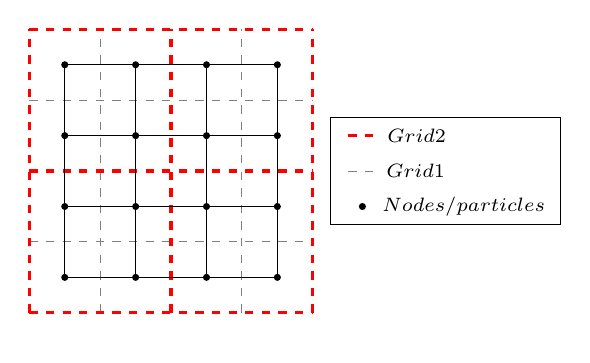
\begin{tikzpicture}[scale=0.9]
  \draw (0,0) --(3,0)--(3,3)--(0,3)--(0,0);
  \draw[white] (0.,0) -- (0,-0.8);
  %%% Grid 1
  \foreach \y in {-0.5,0.5,...,3.5} 
  \draw[dashed,gray] (-0.5,\y) -- (3.5,\y);
  \foreach \x in {-0.5,0.5,...,3.5} 
  \draw[dashed,gray] (\x,-0.5) -- (\x,3.5);
  %%% Grid 2
  \foreach \y in {-0.5,1.5,...,3.5} 
  \draw[dashed,Red,very thick] (-0.5,\y) -- (3.5,\y);
  \foreach \x in {-0.5,1.5,...,3.5} 
  \draw[dashed,Red,very thick] (\x,-0.5) -- (\x,3.5);
  \foreach \y in {0.,1.,...,3.} 
  \foreach \x in {0.,1.,...,3.} 
  \fill (\x,\y) circle(0.05);
  \foreach \y in {0.,1.,...,3.} 
  \draw (0,\y) -- (3.,\y);
  \foreach \x in {0.,1.,...,3.} 
  \draw (\x,0) -- (\x,3);
  \draw (3.75,0.75) rectangle (7.,2.25);
  \fill (4.2,1.) circle (0.05) node [right] {\scriptsize$ \: \: \text{Nodes / particles}$};
  \draw[dashed,gray] (4.,1.5) -- (4.4,1.5) node [right] {\scriptsize$\color{black} \text{Grid 1}$};
  \draw[dashed,very thick,Red] (4.,2.) -- (4.4,2.) node [right] {\scriptsize$\color{black} \text{Grid 2}$};
\end{tikzpicture}


%%% Local Variables:
%%% mode: latex
%%% TeX-master: "../manuscript"
%%% End:
}
  \caption{Geometry, loading and boundary conditions for the tensile impact problem on a two-dimensional elastic medium. The initial velocity is set to $v_d=-200 \: m/s$.}
  \label{fig:PS_domain}
\end{figure}
It is worth noticing that this simulation enables comparisons between the numerical methods in spite of the lack of exact solution for that problem.
Unfortunately, this cannot be circumvented by taking a FEM solution on a very fine mesh as the reference one since, as mentioned in section \ref{sec:plane-strain-problem}, a refinement does not prevent from spurious oscillations and hence, from an overestimation of the plastic strain.



Comparisons of the isovalues of longitudinal PK1 stress $\Pi_{11}$ and cumulated plastic strain $p$ are depicted in figures \ref{subfig:stress_comparison} and \ref{subfig:epls_comparison} respectively for two time steps that correspond to the incident and reflected pressure waves.
The fields are plotted on the current configuration so as to show the deformed shape resulting from each simulation.
Notice that a mesh is reconstructed based on the material points for MPM and DGMPM results for vizualisation purpose.

Before the reflection of the pressure wave, the arising of spurious oscillations arising in MPM and FEM solutions, though much slighter in the latter, and of numerical diffusion in DGMPM(4ppc) one, leads to different assessement of fields.
In addition to the stress peaks occuring in the MPM stress solution in the bottom part of the domain, a checkerboard structure can be seen upstream.
Then, figure \ref{subfig:epls_comparison} shows that the numerical cumulated plastic strains have globally the same shape but different extreme values.

Next, the incident wave reflects on the right end of the solid as a tensile wave so that the bottom part of the boundary starts moving rightward.
After that reflection, similar observations can be made about the MPM and the DGMPM(4ppc) stress solutions, that is, significant oscillations and numerical diffusion respectively.
Moreover, although the FEM and DGMPM(1ppc) stresses are quite similar before the reflection, it is no longer the case after the passage of the tensile wave so that the FEM solution exhibit a maximum that is higher than DGMPM one.
On the other hand, the plastic continues propagating within the domain and no significant difference appears in the numerical cumulated plastic strains.
At that time, it can also be seen that the shapes of the solid domain are quite similar, even though DGMPM solutions leads to a slightly lower vertical displacement of the top left corner of the square.
\begin{figure}[ht]
  \centering
  \subcaptionbox{Stress \label{subfig:stress_comparison}}{\begin{tikzpicture}[scale=1]
  \begin{groupplot}[group style={group size=2 by 4,% columns by rows
      ylabels at=edge left, yticklabels at=edge left,
      horizontal sep=5.ex,
      vertical sep=2ex,},
    enlargelimits=0,
    xmin=0.,xmax=1., ymin=-0.,ymax=1.
    ,axis on top,scale only axis,width=0.18\linewidth
    ,xtick=\empty,ytick=\empty,
    colorbar style={
      title style={
        font=\normalsize,
        at={(1,.5)},
        anchor=north west
      },yticklabel style={font=\normalsize}
      ,at={(current axis.south east)},anchor=south west
    },colormap name=tol
    ]
    %% FIRST ROW (time 1 = 5.10e-4s)
    %%% RANGE -8.6e9 -- 0.57e9
    \nextgroupplot[title={$t=5.10\times 10^{-4} \:s$},ylabel={FEM}]\addplot graphics[xmin=0.,xmax=1., ymin=-0.,ymax=1.] {pngFigures/fem_stress1-crop.png};
    \nextgroupplot[title={$t=1.02\times 10^{-3} \:s$}]\addplot graphics[xmin=0.,xmax=1., ymin=-0.,ymax=1.] {pngFigures/fem_stress2-crop.png};

    \nextgroupplot[ylabel={MPM(1ppc)}]\addplot graphics[xmin=0.,xmax=1., ymin=-0.,ymax=1.] {pngFigures/mpm_stress1-crop.png};
    \nextgroupplot[]\addplot graphics[xmin=0.,xmax=1., ymin=-0.,ymax=1.] {pngFigures/mpm_stress2-crop.png};

    \nextgroupplot[ylabel={DGMPM(1ppc)}]\addplot graphics[xmin=0.,xmax=1., ymin=-0.,ymax=1.] {pngFigures/dgmpm1ppc_stress1-crop.png};
    \nextgroupplot[]\addplot graphics[xmin=0.,xmax=1., ymin=-0.,ymax=1.] {pngFigures/dgmpm1ppc_stress2-crop.png};
    

    \nextgroupplot[ylabel={DGMPM(4ppc)},colorbar horizontal,colorbar  style={
      title style={yshift=-1.5cm},
      title= {$\Pi_{11}\: (GPa)$},
      xtick={-8.6,0.57},
      xticklabels={-8.6,0.57},
    }]
    \addplot[scatter,scatter src=x,mark size=0.pt] coordinates {(-8.6,0.) (0.57,0)};% Fake extreme values to fix scale
    \addplot graphics[xmin=0.,xmax=1., ymin=-0.,ymax=1.] {pngFigures/dgmpm4ppc_stress1-crop.png};
    \nextgroupplot[colorbar horizontal,colorbar  style={
      title style={yshift=-1.5cm},
      title= {$\Pi_{11}\: (GPa)$},
      xtick={-2.3,5.6},
      xticklabels={-2.3,5.6},
    }]
    \addplot[scatter,scatter src=x,mark size=0.pt] coordinates {(-2.3,0.) (5.6,0)};% Fake extreme values to fix scale
    \addplot graphics[xmin=0.,xmax=1., ymin=-0.,ymax=1.] {pngFigures/dgmpm4ppc_stress2-crop.png};
    
  \end{groupplot}
\end{tikzpicture}



%%% Local Variables:
%%% mode: latex
%%% TeX-master: "../manuscript"
%%% End:
}\qquad
  \subcaptionbox{Cumulated plastic strain \label{subfig:epls_comparison}}{\begin{tikzpicture}[scale=1]
  \begin{groupplot}[group style={group size=2 by 4,% columns by rows
      ylabels at=edge left, yticklabels at=edge left,
      horizontal sep=5.ex,
      vertical sep=2ex,},
    enlargelimits=0,
    xmin=0.,xmax=1., ymin=-0.,ymax=1.
    ,axis on top,scale only axis,xtick=\empty,ytick=\empty,width=0.18\linewidth,
    colorbar style={
      title style={
        font=\normalsize,
        at={(1,.5)},
        anchor=north west
      },yticklabel style={font=\normalsize}
      ,at={(current axis.south east)},anchor=south west
    },colormap name=tol]
    %% FIRST ROW (time 1 = 5.10e-4s)
    %%% RANGE -8.6e9 -- 0.57e9
    \nextgroupplot[title={$t=5.10\times 10^{-4} \:s$},ylabel={FEM}]\addplot graphics[xmin=0.,xmax=1., ymin=-0.,ymax=1.] {pngFigures/fem_epeq1-crop.png};
    \nextgroupplot[title={$t=1.02\times 10^{-3} \:s$}]\addplot graphics[xmin=0.,xmax=1., ymin=-0.,ymax=1.] {pngFigures/fem_epeq2-crop.png};

    \nextgroupplot[ylabel={MPM(1ppc)}]\addplot graphics[xmin=0.,xmax=1., ymin=-0.,ymax=1.] {pngFigures/mpm_epeq1-crop.png};
    \nextgroupplot[]\addplot graphics[xmin=0.,xmax=1., ymin=-0.,ymax=1.] {pngFigures/mpm_epeq2-crop.png};

    \nextgroupplot[ylabel={DGMPM(1ppc)}]\addplot graphics[xmin=0.,xmax=1., ymin=-0.,ymax=1.] {pngFigures/dgmpm1ppc_epeq1-crop.png};
    \nextgroupplot[]\addplot graphics[xmin=0.,xmax=1., ymin=-0.,ymax=1.] {pngFigures/dgmpm1ppc_epeq2-crop.png};
    

    \nextgroupplot[ylabel={DGMPM(4ppc)},colorbar horizontal,colorbar  style={
      title style={yshift=-1.5cm},
      title= {$p$},
      xtick={0,.15},
      xticklabels={0,0.15},
    }]
    \addplot[scatter,scatter src=x,mark size=0.pt] coordinates {(0,0.) (0.15,0)};% Fake extreme values to fix scale
    \addplot graphics[xmin=0.,xmax=1., ymin=-0.,ymax=1.] {pngFigures/dgmpm4ppc_epeq1-crop.png};
    \nextgroupplot[colorbar horizontal,colorbar  style={
      title style={yshift=-1.5cm},
      title= {$p$},
      xtick={0.,0.16},
      xticklabels={0,0.16},
    }]
    \addplot[scatter,scatter src=x,mark size=0.pt] coordinates {(0.,0.) (0.16,0)};% Fake extreme values to fix scale
    \addplot graphics[xmin=0.,xmax=1., ymin=-0.,ymax=1.] {pngFigures/dgmpm4ppc_epeq2-crop.png};
    
  \end{groupplot}
\end{tikzpicture}



%%% Local Variables:
%%% mode: latex
%%% TeX-master: "../manuscript"
%%% End:
}
  \caption{Isovalues of the PK1 stress tensor component $\Pi_{11}$ and cumulated plastic strain in a two-dimensional hyperelastic-plastic solids impacting a rigid wall under plane strain. Comparison of FEM (CFL=0.9), MPM (CFL=0.7) and DGMPM solutions using either one particle per cell (CFL=1) or four particles per cell (CFL=0.4).}
  \label{fig:PS_taylor}
\end{figure}

We now propose to look at the above results in more details.
Figures \ref{fig:bottom_line} and \ref{fig:left_line} show the evolution of longitudinal stress and cumulated plastic strain along the bottom and left end of the domain respectively for the same time steps.
First, it can be seen in figure \ref{subfig:bottom1} that the incident wave is described with different level of sharpness by the numerical shemes.
% Note however that no elastic predictor is seen in the stress profiles in contrast to the one-dimensional problem studied above.
Then, the figure also shows the oscillations in the MPM stress solution mentioned above.
Moreover, the superimposition of the stresses resulting from MPM computations using 1ppc or 4ppc shows that refining the particles discretization does not allow removing the numerical noise.
As a consequence, the numerical cumulated plastic strains near the wave front are rather different since the solutions of particle-based methods are ahead of the FEM one.
Upstream that front, the MPM(1ppc) plastic strain exhibits some peaks while this computed with the MPM(4ppc) is closer to the finite element solution.
On the other hand, the two space discretizations lead to DGMPM results that are close from one to another on the plastic plateau.

After the reflection (figure \ref{subfig:bottom2}), the stress profiles are much more different.
The MPM still yields oscillating solutions regardless the space discretization used, and DGMPM results are smoother than the other.
Once Again, the FEM leads to a rather sharp solution.
\begin{figure}[ht]
  \centering
  {\phantomsubcaption{\label{subfig:bottom1}}}
  {\phantomsubcaption{\label{subfig:bottom2}}}
  \begin{tikzpicture}
  \begin{groupplot}[group style={group size=2 by 2, % 3 columns 2 rows
      ylabels at=edge left, yticklabels at=edge left,horizontal sep=2.ex,vertical sep=5.ex,
      xticklabels at=edge bottom,xlabels at=edge bottom},
    ymajorgrids=true,xmajorgrids=true,
    axis on top,scale only axis,width=0.425\linewidth, every x tick scale label/.style={at={(xticklabel* cs:1.05,0.75cm)},anchor=near yticklabel},
    every y tick scale label/.style={at={(yticklabel* cs:1.05,-.9cm)},anchor=near yticklabel}]
    
    %%%%%%%%%%%%%%%%%%%% 
    % ============================== Stress Line
    % t1 
    \nextgroupplot[ylabel=$\Pi_{11} \:(Pa)$,title={(a) $t = 5.10 \times 10^{-4}\: s$},ymin=-1.e10,ymax=7.25e9]
    \addplot[Orange,thick,mark=*,mark repeat=2] table[x=Points:0,y=Piola_Stress:0] {csvFiles/fem_bottom1.csv};
    \addplot[Red,thick,mark=square,only marks] table[x=Points:0,y=Piola:0] {csvFiles/mpm_bottom1.csv};
    \addplot[black!60,thick,mark=o,only marks] table[x=Points:0,y=Piola:0] {csvFiles/mpm4ppc_bottom1.csv};
    \addplot[Blue,thick,mark=asterisk,only marks,mark size=3pt] table[x=Points:0,y=PK1:0] {csvFiles/dgmpm1ppc_bottom1.csv};
    \addplot[Purple,thick,mark=x,only marks,mark size=3pt,mark repeat=2] table[x=Points:0,y=PK1:0] {csvFiles/dgmpm4ppc_bottom1.csv};
    
    % t2 
    \nextgroupplot[title={(b) $t = 1.02 \times 10^{-3}\: s$},ymin=-1.e10,ymax=7.25e9%,ymin=-7.5e9,ymax=100.e9,ytick scale label code/.code={},legend style={at={($(0.75,-0.4)+(0.9cm,0.6cm)$)},legend columns=3}
    ]
    \addplot[Orange,thick,mark=*,mark repeat=2] table[x=Points:0,y=Piola_Stress:0] {csvFiles/fem_bottom2.csv};
    \addplot[Red,thick,mark=square,only marks] table[x=Points:0,y=Piola:0] {csvFiles/mpm_bottom2.csv};
    \addplot[black!60,thick,mark=o,only marks] table[x=Points:0,y=Piola:0] {csvFiles/mpm4ppc_bottom2.csv};
    \addplot[Blue,thick,mark=asterisk,only marks,mark size=3pt] table[x=Points:0,y=PK1:0] {csvFiles/dgmpm1ppc_bottom2.csv};
    \addplot[Purple,thick,mark=x,only marks,mark size=3pt,mark repeat=2] table[x=Points:0,y=PK1:0] {csvFiles/dgmpm4ppc_bottom2.csv};


    % ============================== Cumulated plastic strain Line
    % t1 
    \nextgroupplot[ylabel=$p$,xlabel=$x \: (m)$,ymin=0.,ymax=9.e-2%,ymin=-7.5e9,ymax=100.e9,ytick scale label code/.code={}
    ]
    \addplot[Orange,thick,mark=*,mark repeat=2] table[x=Points:0,y=Equivalent_Plastic_Strain] {csvFiles/fem_bottom1.csv};
    \addplot[Red,thick,mark=square,only marks] table[x=Points:0,y=epeq] {csvFiles/mpm_bottom1.csv};
    \addplot[black!60,thick,mark=o,only marks] table[x=Points:0,y=epeq] {csvFiles/mpm4ppc_bottom1.csv};
    \addplot[Blue,thick,mark=asterisk,only marks,mark size=3pt] table[x=Points:0,y=epeq] {csvFiles/dgmpm1ppc_bottom1.csv};
    \addplot[Purple,thick,mark=x,only marks,mark size=3pt,mark repeat=2] table[x=Points:0,y=epeq] {csvFiles/dgmpm4ppc_bottom1.csv};
    
    % t2
    \nextgroupplot[legend style={at={($(0.75,-0.35)+(0.cm,1cm)$)},legend columns=5},xlabel=$x \: (m)$,ymin=0.,ymax=9.e-2%,ymin=-7.5e9,ymax=100.e9,ytick scale label code/.code={}
    ]
    \addplot[Orange,thick,mark=*,mark repeat=2] table[x=Points:0,y=Equivalent_Plastic_Strain] {csvFiles/fem_bottom2.csv};
    \addplot[black!60,thick,mark=o,only marks] table[x=Points:0,y=epeq] {csvFiles/mpm_bottom2.csv};
    \addplot[Red,thick,mark=square,only marks] table[x=Points:0,y=epeq] {csvFiles/mpm4ppc_bottom2.csv};
    \addplot[Blue,thick,mark=asterisk,only marks,mark size=3pt] table[x=Points:0,y=epeq] {csvFiles/dgmpm1ppc_bottom2.csv};
    \addplot[Purple,thick,mark=x,only marks,mark size=3pt,mark repeat=2] table[x=Points:0,y=epeq] {csvFiles/dgmpm4ppc_bottom2.csv};

    \addlegendentry{fem \:}
    \addlegendentry{mpm (1ppc) \:}
    \addlegendentry{mpm (4ppc) \:}
    \addlegendentry{dgmpm (1ppc) \:}
    \addlegendentry{dgmpm (4ppc) \:}
    
    
  \end{groupplot}
\end{tikzpicture}



%%% Local Variables:
%%% mode: latex
%%% TeX-master: "../manuscript"
%%% End:

  \caption{Comparison of the longitudinal stress component and cumulated plastic strain along the bottom boundary of the domain at two times.}
  \label{fig:bottom_line}
\end{figure}
Furthermore, the MPM cumulated plastic strain curves oscillate around the FEM one which, in turn, is above these computed with the DGMPM.

The above observations are even more significant when looking at the evolution of fields along the left end of the square (figure \ref{fig:left_line}).
In figure \ref{subfig:left1}, FEM and DGMPM stress profiles show good agreement while spurious oscillations pollute MPM ones. 
Although FEM and DGMPM stresses are similar, it is not the case for the cumulated plastic strains for which the numerical results differ more.
Thus, the MPM yields the highest values of cumulated plastic strain at the top left corner of the domain.
The results depicted at the subsequent time show tremendous oscillations in the MPM(1ppc) solution for which the longitudinal stress varies roughly from $-7 \: GPa$ to $1 \: GPa$ in the bottom part of the left boundary.
These oscillations are reduced, though not completely removed, in the MPM(4ppc) results. 
On the other hand, DGMPM and FEM solutions no longer fit.
\begin{figure}[ht]
  \centering
  {\phantomsubcaption{\label{subfig:left1}}}
  {\phantomsubcaption{\label{subfig:left2}}}
  \input{pgfFigures/left_line}
  \caption{Comparison of the longitudinal stress component and cumulated plastic strain along the left boundary of the domain at two times.}
  \label{fig:left_line}
\end{figure}
It appears that the stress curve corresponding to the latter is bounded by these of the DGMPM(4ppc) and DGMPM(1ppc), the lower bound being given by the single particle space discretization.
At last, the cumulated plastic strain curves show similar behaviors to those of the previous time step except close to the bottom left corner of the domain.
In that region, the plastic flow developed differently depending on the numerical solution considered.
Both DGMPM curves are below that computed with the FEM while the profiles resulting from MPM computations are less regular than the other.

\subsection{Non-linear hardening material}
\label{sec:non-linear-hardening}
Reprendre le cas test hyperelastique de la these?


%%% Local Variables:
%%% mode: latex
%%% TeX-master: "manuscript"
%%% End:


\section{Towards a two-dimensional elastoplastic Riemann solver}
\label{sec:ep_Riemman_solver}
Commencer par un résumé du ce qui a été identifié au dessus.

Eventuellement ne parler que d'un cas pour lequel c'est plus simple comme les defs planes (encore que...).

On pourrait faire comme Lin et Ballman \cite{Lin_et_Ballman} en se donnant 3 composantes de contraintes et en intégrant. 
C'est ce qui paraît le plus faisable dans l'état. 
Sauf que sigma22 fout la merde à cause car on a 3 inconnues en contraintes alors que pour le thin-walled tube on en n'avait que 2 et on pouvait itérer comme ça.
En effet, les interscetions dans les plans u,sigma et v,tau des courbes intégrales nous donnait des nouveaux états de contraintes pour l'étape d'après. 
Qu'en est-il avec sigma22 ?


Pour un solveur approximé:
Identifier le trajet ?? A priori, on ne peut pas sans intégrer.
Sauf si on fait une projection radiale de l'état trial sur le critère et qu'on cherche quelle onde part de là.
Il semblerait tout de même que la plasticité est surtout répendue par les ondes slow.
Les ondes fast font tourner autour du critère. 
Clifton suppose qu'elles n'existent que si leurs point de départ est à tau=0. On peut faire la même chose ?
On peut approximer les trajets par la tangente sur le critère pour les ondes slow.
%% Tracer des structures charactéristiques (revoir dans la biblio où on met une discontinuité et où on n'en met pas)








%%% Local Variables:
%%% mode: latex
%%% TeX-master: "../mainManuscript"
%%% End:



\section*{Conclusion}

In this chapter, the characteristic structure of the solution of hyperbolic problems in elastic-plastic solids in two space dimensions has been highlighted.
It is known since the 50s that plastic flow in two-dimensional solids yields two families of waves which speeds depend on the stress state, the slow and fast waves.
As a result, shock and simple waves may occur in an elastoplastic medium even for linear hardening material.
In addition, these plastic waves may have an impact on several stresses in contrast to elastic discontinuities across which one stress component varies, hence the name of combined stress waves.
During the 60s, attention has been paid to simple waves in particular two-dimensional problems thus providing, among other, solutions of Picard problems in elastic-plastic medium undergoing step loadings \cite{Clifton,Ting68,Ting73}. % Idem pour ting ? c'est dit dans l'intro ? voir ce qui est fait dans le 73
The singular nature of such problems lies in the fact that the characteristic structure of the solution depends on the external loading undergone.
Indeed, it has been shown \cite{Clifton} that boundary conditions can lead to plastic flow involving one fast, one slow, or both simple waves.
Therefore, it is crucial to be able to identify typical stress paths followed in each simple waves in order to link the initial data to a given stress state, and subsequently to determine the occurring wave pattern.

$\newline$
%% Lin et Ballman
Based on those works, an iterative Riemann solver \cite{Lin_et_Ballman}, which procedure has been recalled in section \ref{sec:stress_paths_num}, has been developed for the numerical solution of the thin-walled tube problem. 
% L'idée ici c'est de généraliser cette approche pour tous les problèmes 2D
Following this approach, identifying characteristic wave patterns for general elastoplastic problems in two space dimensions should allow to enrich the numerical solution with the knowledge of physics.
For that purpose, the characteristic analysis of two-dimensional problems in elastic-plastic materials with linear isotropic hardening under plane strain and plane stress, in projection in an arbitrary direction of space, has been carried out in section \ref{sec:charac_plast}.
Fast and slow waves are also involved in the solution so that applying the method of characteristic through the simple waves provides a system of ODE.
Integration of this system leads to combined stress paths that are followed between initial and final stress states on the one hand, and to the integral curves in terms of velocity components involving integral along those loading paths on the other hand.
Specializing the ODEs to one direction of a Cartesian grid, it has been shown in section \ref{sec:stress_paths} that the loading paths satisfied through slow and fast waves are perpendicular in the stress space for both plane strain and plaen stress.
Moreover, it has been established that the stress paths exhibit particular behavior in the space $(\sigma_{11},\sigma_{22},\sigma_{12})$, that is $d\sigma_{11}=0$, $d\sigma_{12}=0$ or $d\sigma_{22}=0$, for special values of the components of the acoustic tensor.
These situations are achieved for different stress states depending on wheter the problem involves plane stresses of plane strains as shown in section \ref{sec:stress_paths}.

$\newline$
The complexity of the ODEs derived in section \ref{sec:charac_plast} prevents from identifying all the singularities which may occur along the loading paths.
Hence, the mathematical analysis has been supplemented with numerical results consisting in the integration of stress paths from arbitrary initial stress values lying on the initial yield surface, for the particular direction of space $\vect{e}_1$.

%% Thin-walled tube
First, in section \ref{sec:num_thin-walled} the loading paths resulting from the integration of the ODEs derived in section \ref{sec:charac_plast} have been compared to those of Clifton \cite{Clifton}.
The two different formulations, respectively based on elastoplastic stiffnesses and softnesses, show a good agreement.

%% Cont. planes
Second, some the evolution of stress components across fast and slow waves under plane stress has been looked at in section \ref{sec:num_plane_stress}.
It appears that though the loading paths are rather complex in stress space through a fast wave, the stress evolution in the deviatoric plane is restricted to the initial yield surface until one direction of pure shear is reached.
A singularity then occurs so that the numerical integration cannot be pursued.
On the other hand, the loading paths resulting from the integration of ODEs satisfied inside a slow wave, except that $\sigma_{11}$ varies much less than the other stress components.

%% Def. planes
Third, the plane strain case has been considered in section \ref{sec:num_plane_strain}.
Once again, the integral curves inside a fast wave show complex shapes in stress space, and an evolution restricted to the initial yield surface in the deviatoric plane.
In that case, however, the paths may follow a direction of pure tensile/compression in the latter plane so that the plastic flow is radial. 
In contrast, the slow waves lead to a stress state of pure shear in the deviatoric plane.

%%% Local Variables:
%%% mode: latex
%%% TeX-master: "../mainManuscript"
%%% End:
